% This must be in the first 5 lines to tell arXiv to use pdfLaTeX, which is strongly recommended.
\pdfoutput=1
% In particular, the hyperref package requires pdfLaTeX in order to break URLs across lines.

\documentclass[11pt]{article}

% Change "review" to "final" to generate the final (sometimes called camera-ready) version.
% Change to "preprint" to generate a non-anonymous version with page numbers.
% \usepackage[review]{acl}
% fixed for camera-ready
\usepackage[final]{acl}

% Standard package includes
\usepackage{times}
\usepackage{latexsym}

% For proper rendering and hyphenation of words containing Latin characters (including in bib files)
\usepackage[T1]{fontenc}
% For Vietnamese characters
% \usepackage[T5]{fontenc}
% See https://www.latex-project.org/help/documentation/encguide.pdf for other character sets

% This assumes your files are encoded as UTF8
\usepackage[utf8]{inputenc}

% This is not strictly necessary, and may be commented out,
% but it will improve the layout of the manuscript,
% and will typically save some space.
\usepackage{microtype}

% This is also not strictly necessary, and may be commented out.
% However, it will improve the aesthetics of text in
% the typewriter font.
\usepackage{inconsolata}

%Including images in your LaTeX document requires adding
%additional package(s)
\usepackage{graphicx}
\usepackage{subcaption}

% % by Sumin
% \usepackage{pifont}
% \usepackage{multirow}
\usepackage{booktabs}
\usepackage{amssymb,amsmath,amsthm}
\usepackage{bm}
\usepackage{pifont}
\usepackage{multirow}
% \usepackage{subfigure}
\setlength{\abovedisplayskip}{10pt} % Space above equations
\setlength{\belowdisplayskip}{10pt} % Space below equations



\newcommand{\etal}{\textit{et al}. }
\newcommand{\ie}{\textit{i}.\textit{e}., }
\newcommand{\eg}{\textit{e}.\textit{g}., }

\newcommand{\phseo}[1]{\textcolor{blue}{[Paul: #1]}}
\newcommand{\sumin}[1]{\textcolor{orange!85!black}{[Sumin: #1]}}
\newcommand{\junyoung}[1]{\textcolor{purple}{[Junyoung: #1]}}
\newcommand{\chanjun}[1]{\textcolor{red}{[Chanjun: #1]}}
\newcommand{\model}{LCIRC}

% If the title and author information does not fit in the area allocated, uncomment the following
%
%\setlength\titlebox{<dim>}
%
% and set <dim> to something 5cm or larger.

\title{LCIRC: A Recurrent Compression Approach for Efficient Long-form Context and Query Dependent Modeling in LLMs}

% fixed for camera-ready
\author{
Sumin An\textsuperscript{1} \qquad
Junyoung Sung\textsuperscript{1} \qquad
Wonpyo Park\textsuperscript{2}
\\
\textbf{Chanjun Park\textsuperscript{1,\(\dagger\)}} \qquad
\textbf{Paul Hongsuck Seo\textsuperscript{1,\(\dagger\)}}
\\
\textsuperscript{1}Dept. of CSE, Korea University
\qquad
\textsuperscript{2}Google
\\
\texttt{\{suminan, jys7451, bcj1210, phseo\}@korea.ac.kr}
\\
\texttt{wppark@google.com}
}


\begin{document}
\maketitle
\begin{abstract}
While large language models (LLMs) excel in generating coherent and contextually rich outputs, their capacity to efficiently handle long-form contexts is limited by fixed-length position embeddings. Additionally, the computational cost of processing long sequences increases quadratically, making it challenging to extend context length. 
To address these challenges, we propose Long-form Context Injection with Recurrent Compression (LCIRC), a method that enables the efficient processing long-form sequences beyond the model's length limit through recurrent compression without retraining the entire model.
We further introduce query dependent context modeling, which selectively compresses query-relevant information, ensuring that the model retains the most pertinent content. Our empirical results demonstrate that Query Dependent LCIRC (QD-LCIRC) significantly improves LLM's ability to manage extended contexts, making it well-suited for tasks that require both comprehensive context understanding and query relevance.

\end{abstract}
% fixed for camera-ready
\let\thefootnote\relax\footnotetext{$^\dagger$Co-corresponding authors.}

\documentclass[../main.tex]{subfiles}
\graphicspath{{../images/}}
\makeatletter
\def\input@path{{../images/}}
\makeatother
\begin{document}
\section{Introduction}
\begin{figure}
\centering
\begin{tikzpicture}
\node[inner sep=0pt] (ws) at (0, 0) {
\includegraphics[height=.4\textwidth, trim={10cm 0 10cm 0},clip]{world_space.png}};
\node[inner sep=0pt] (cs) at (6,0) {\includegraphics[height=.4\textwidth, trim={10cm 1cm 10cm 4cm},clip]{conf_space.png}};
\end{tikzpicture}
\vspace{-5pt}
\label{fig:pbrm_intro}
\caption{\textbf{Left}: Shows world space obstacles as grey spheres. Robots start and goal configuration is colored red and green, respectively. Configurations along the computed path are colored transparent blue. \textbf{Right:} Mapped world space scenario to configuration space. Obstacle region is the grey mesh. Red spheres are collision-free regions computed by the neural SCDF. The optimized shortest path in the convex corridor is the blue curve.}
\vspace{-25pt}
\end{figure}
Motion planning is the problem of finding a collision-free trajectory that connects a given start and goal configuration. The planning takes place in the configuration space of the robot. For single body robots, like mobile robots or drones, the configuration space and the world space are usually the same. This simplifies the planning, since explicit obstacle representations are available which enables geometrical tools like separating hyperplanes, smallest distance to obstacles etc., to be used when designing motion planning algorithms. For multi-body robots like manipulators, the situation is completely different. The world space obstacles are usually mapped to non-convex regions, and to make the problem even harder, the mapping is usually not known. Forming explicit representations of the obstacle region in the configuration space is usually too expensive or intractable. Despite all of this, sampling based planners are used with great success, which mainly is due to their use of implicit representations of the obstacle region. The basic idea is to construct a graph in the configuration space that covers and connects the collision-free region. From this graph, a path can be extracted that connects a given start and goal configuration. The approach is computationally expensive, since the graph is constructed with the smallest geometrical building block available, points, which represents a collision-check. Furthermore, the extracted paths from the graph are non-smooth and jagged due to the stochastic nature of the approach. This adds an additional post-processing step to the process, where the paths are shortcutted and smoothened, before the path can be used for tracking. Clearly a lot of time is invested to form this graph and produce smooth paths. Thus, if the obstacles start to move, then all of this work is done in no use, since all points that make up this graph need to be re-verified, which is simply too time consuming to be done in real time.
\\\\
In this work, we want to address the existing drawbacks of the sampling based planners. Our main contribution is an improved motion planner where each vertex in the graph covers a collision-free region in the form of a sphere instead of a point and where the edges are formed with neighboring intersecting spheres. This representation has the advantage of instead of returning piecewise linear paths, returning a sequence of overlapping spheres, i.e. a convex corridor, that connects a given start and goal configuration, illustrated in Figure \ref{fig:pbrm_intro}. This convex corridor allows us to use convex optimization to produce smooth trajectories, instead of computationally expensive post-processing methods. The representation further allows us to estimate the coverage of the collision-free space, which gives us awareness and feedback in the offline roadmap construction phase. Finally, our representation is simple to adapt to moving obstacles, simply requery for the new radii and recheck for intersections. 
\\\\
The spherical collision-free regions are formed using a signed distance function (SDF), which is a function that returns the smallest distance from an arbitrary point to the boundary of an obstacle. As the name implies, the distance is signed, thus if the point is inside the obstacle it is negative otherwise positive. If the distance is positive, a sphere with radius equal to the distance is guaranteed to cover a collision-free region. Using an SDF in motion planning is not new, but what is novel about our approach is that we express the distance in the configuration space instead of the world space and by doing so allows us to form these convex collision-free regions. We refer to the resulting SDF as a signed configuration distance function (SCDF). Computing an SCDF analytically is non-trivial, our approach is therefore to parameterize the SCDF with a deep neural network and learn the mapping by supervised learning. Our resulting neural SCDF can compute distances for different parameter values of obstacle shapes and we also show how multiple distances can be combined, thus making our approach flexible.
\section{Related work}
Motion planning algorithms can roughly be divided into three families, grid-based, sampling based and optimization based methods. Grid-based methods (GBM) discretize the planning space from which a graph is then compiled. A standard search method is A$^\star$ \citep{a_star}, which is classified as an \textit{informed} search method, since it employs a heuristic function to speed up the search. A$^\star$ guarantees to return an optimal path at the level of discretization used. GBMs usually discretize the planning space by a regular lattice and this limits the GBMs to problems with low dimensionality due to the curse of dimensionality. Thus, GBMs are usually limited to single-body robots where the degrees of freedom (DOF) are low. To overcome the inherent scaling problem with the GBMs, stochastic methods are usually used for multi-body robots. These methods are termed as sampling-based methods (SBM) and core members within this family are the rapidly-exploring random trees (RRT) \citep{rrt} and the probabilistic roadmap (PRM) \citep{prm}. RRT grows a tree from the start configuration and explores the collision-free region in a rapid way until it is able to connect to the goal region. RRT is usually improved by bi-directional planning \citep{rrt_connect}, i.e. an additional tree is grown from the goal configuration and the trees are tested for connection after any tree has been expanded. RRT is a single-query method, thus it searches for a path from scratch each time it is queried. Contrary to this, PRM is a multi-query method, which solves for multiple queries without starting from scratch. PRM does this by creating a roadmap (graph) that covers the collision-free space as an offline step. The graph is then used to solve for multiple queries. PRMs are used in cases where the environment does not change since the extra offline step is too computationally costly and needs to be re-done if the environment is changed. In our work, we address this inherent issue by using a different roadmap representation. Our vertices in the graph cover a collision-free region in the form of spheres and we form the edges by checking for intersecting spheres. If something in the environment changes, we recompute the spheres radii and recheck the intersections, without relying on collision detection. We use a trained neural network to compute the sphere radius, therefore querying for the radius can be done fast, hence our representation enables the PRM for dynamic environments.
\\\\
In the recent decades, optimization based methods (OBM) \citep{chomp, schulman, itomp, stomp} have been introduced as an alternative to SBM for multi-body robots. Like the SBM, the OBMs scale well to higher dimensional problems and produce smoother motion. It is common to use a SDF in the optimization since it is a smooth function, thus enabling gradient-based methods. However, the standard way of expressing the SDF is in world space. The distance therefore needs to be mapped to the configuration space by the forward kinematics. This mapping makes the optimization problem a non-linear program (NLP), which is computationally expensive to solve. Recently, a different approach has been proposed. In \cite{mp_gcs} motion planning is formulated as a convex optimization problem by using the graph of convex sets framework \citep{gcs}. The underlying idea is to decompose the collision-free space into intersecting convex sets from which a convex optimization problem is formulated. In cases where an explicit representation of the obstacles in the configuration space exists, like for single-body robots, creating collision-free convex regions can be done fast \citep{iris}. For multi-body robots, this is non-trivial. Existing work does this successfully \citep{iris_nlp, iris_c} by an optimization based approach, but the methods are still too time consuming to be used in the presence of moving obstacles. Our approach is instead to use deep learning to learn an SDF expressed in the configuration space. With this, we can query for shortest distances to the collision boundary, which allows us to expand spherical regions which are collision-free. Our approach is fast and therefore enables our suggested roadmap planner to be used in dynamic environments.
\\\\
Recent research has focused on learning collision detection \citep{fk_kernel_distance, diffco, graphdistnet} by predicting the signed distance between the robot links and the surrounding obstacles in the world space. The learned SDF is used in trajectory optimization but since the distance is expressed in the world space, the problem becomes an NLP and therefore takes a long time to solve. We take a novel approach and suggest to instead express the signed distance in the configuration space. This allows us to improve the PRM at the same time as it enables convex optimization for trajectory optimization, which runs faster and is more reliable than NLP solvers. In \cite{cspf} a learned signed distance function in the configuration space is proposed similar to our approach. However, their approach is restricted to point cloud representations, while we propose to represent the obstacles as parameterized geometric shapes, e.g. spheres. Furthermore, we also show how to use our learned SCDF to improve an existing roadmap planner.
\section{Problem formulation}
A robot is located in the world space, $\W \subset \R^3 $. The unique location of the robot is given by its configuration $\q \in \C$, where $\C$ is the configuration space. The set of points covered by the robots bodies at a certain configuration is expressed as $\B(\q) \subset \W$. The robot is surrounded by $\NrObst$ obstacles $\O = \bigcup_{i=1}^{\NrObst} \O_i$, where  $\O_i \subset \W$. The representation of the obstacle in the configuration space is the set $\C\O_i = \{\q \in \C \: |\: \B(\q) \cap \O_i \neq \emptyset \}$. The obstacle space is formed as $\Co = \bigcup_{i=1}^{\NrObst} \C \O_i$. The complement is referred to as the free space, $\Cf = \C \setminus \Co$. The path planning problem is a tuple, ($\Cf$, $\qStart$, $\qGoal$), where we want to connect a query pair, consisting of a start, $\qStart$, and goal configuration, $\qGoal$, with a geometric path, $\q(s): [0, 1] \mapsto \Cf$, such that $\q(0)=\qStart$ and $\q(1)=\qGoal$, or report correctly when such a path does not exist.
\end{document}

\section{Related Work}
% \subsection{Vision Language Model}
% 시각장애인에서 상황을 설명할 DB가 없으니 만들었다. 그리고 이를 VLM에 튜닝했다.
\subsection{Technical approaches for assisting the visually-impaired}


\subsection{Datasets for visual instruction tuning}

% \begin{figure*}[t]
\centering
\includegraphics[width=\textwidth]{images/pixelmllms_failures/failures_pixmllms_3.drawio.pdf}
\vspace{-2em}
\caption{Second shortcoming of pixel-level MLLMs is the degraded performance in pixel-level visual grounding in certain models. The predicted segmentation is highlighted in red.} 
\label{fig:shortcoming3}
\vspace{-1em}
\end{figure*}

\begin{figure}[t]
\centering
\includegraphics[width=0.5\textwidth]{images/pixelmllms_failures/failures_pixmllms_2.drawio.pdf}
\vspace{-2em}
\caption{Third shortcoming of pixel-level MLLMs is the degraded performance in instruction following, where the question is instructing the model to generate one letter from the options.} 
\label{fig:shortcoming2}
\vspace{-1em}
\end{figure}

In this section, we describe our two benchmarks and probing techniques for pixel-level MLLMs and MLLMs that were not trained with pixel-level grounding supervision.
\subsection{Benchmarks}
\textbf{PixMMVP benchmark:} We build upon the recently released MMVP~\cite{tong2024eyes} which identified clip blind pairs and used them to build a challenging benchmark with the corresponding questions and choices for 300 images. We augment the aforementioned dataset and manually annotate each question with the corresponding object of interest referring expression, e.g. an elderly person or the butterfly's feet. There are seven questions only that are not designed to inquire about a specific object in the scene, which are excluded. Examples include questions inquiring on the view direction of the camera which are not tied to a specific entity. Our manual referring expression annotations are as fine-grained as possible. These expressions correspond to what needs to be grounded in the image to answer the question. Afterwards, we manually label these objects of interest with polygonal annotations using the VGG annotator~\cite{dutta2016via}.

\textbf{PixCV-Bench benchmark:} For this benchmark we build upon the 2D component of the recently released CV-Bench~\cite{tong2024cambrian}. We specifically select the 2D component, since they are sourced from segmentation datasets (i.e., ADE20K~\cite{zhou2017scene} and COCO~\cite{lin2014microsoft}), which can be used in our proposed benchmark. However, the publicly released CV-Bench does not identify the objects in question and their corresponding segmentation. As such we use GPT-4o to parse the questions and identify the objects of interest automatically, followed by manual inspection and correction. Specifically, we collect the classes in each image from the corresponding dataset and construct a list of class choices ``1. $<$CLS1$>$, 2. $<$CLS2$>$, ...''. Then we prompt GPT-4o with the following, \textit{``Provide number only as an answer. Identify the objects of interest in the following question: $<$QUESTION$>$ ? 1. $<$CLS1$>$, 2. $<$CLS2$>$, ... ''.}  This provides us with the categories per question that highlights the objects of interest. While seemingly these are categorical annotations not referring expressions, certain scenarios in CV-Bench are different. Specifically, in the relative positioning task all the questions that include an object highlighted by a red box in the image are annotated with the referring expression, ``(annotated by the red box)'', beyond simple categorical annotations.

Afterwards, we use the selected categories from GPT-4o to retrieve the corresponding segmentation mask/s per image. Furthermore, we use a custom annotation tool to manually filter the objects in the question, e.g. selecting only the object mask annotated by the red box when referred to it and filtering out the other instances for that same class. Another example that needs manual filtration when the class in question is a broader category than what is inquired upon, e.g., ``Pendant Lamp'' which is under the category of ``Lamp'' in ADE20K. In such a case, we filter out the masks of other types such as ``Table Lamp''. Moreover, we identify missing annotations in rare occasions that require additional intervention and manually annotate these missing objects. We provide the final PixCV-Bench with referring expressions and their segmentation annotations that can be used to evaluate the grounding ability in relation to the original VQA task. Appendix~\ref{app:impdetails} provides visual examples from our benchmarks.

\subsection{A Pixel-level MLLMs study}

We utilize the two proposed benchmarks, PixMMVP and PixCV-Bench, to evaluate how the current trend in pixel-level MLLMs that relies on training with grounding supervision perform in such challenging tasks. Furthermore, we inspect the failures of these pixel-level MLLMs and explore simple approaches to pixel-level understanding from MLLMs that overcome the previous shortcomings. %We aim to answer two major research questions in our study; ``How do Pixel-level MLLMs perform in challenging pixel-level visual grounding tasks?'' and ``Whether grounding can be extracted from MLLMs that were not necessarily trained with full supervision as a simpler but more powerful means? and When does that grounding emerge?''

\textbf{Pixel-level MLLMs shortcomings.} We highlight the failures for the current state-of-the-art pixel-level MLLMs through three probing techniques. First, we highlight the degraded performance in VQA from most of the pixel-level MLLMs that are trained with pixel-level grounding supervision. We use for that the following prompt, \textit{``$<$IMG$>$$<$QUESTION$>$? $<$OPTION1$>$ $<$OPTION2$>$...''}, as shown in Figure~\ref{fig:shortcoming1}. Certain pixel-level MLLMs tend to answer the aforementioned question while outputting a corresponding segmentation mask/s for the objects of interest. Notably, the worst two models in this task, LISA~\cite{lai2024lisa} and GLAMM~\cite{rasheed2024glamm}, are not able to provide an answer and rather refer to a segmentation mask. On the other hand, OMG-Llava~\cite{zhang2024omg} shows better ability in VQA.%, yet the answer is not necessarily the correct one.

The second shortcoming we discuss is their degraded ability to visually ground objects. Surprisingly, although they were trained with pixel-level grounding supervision, not all of these models show superior grounding performance. Figure~\ref{fig:shortcoming3} shows the second prompt to generate a segmentation mask for the ground-truth referring expression. The purpose of this probing is to understand whether the failure in these models is purely on the VQA task, or its inability to ground the objects of interest in the corresponding question or both. Figure~\ref{fig:shortcoming3} shows the worst two models in this aspect, which are GLAMM, the region captioning variant, and Llava-G. Both fail to segment the specific object in question, while OMG-Llava shows better performance.

Third, we highlight another shortcoming, where these MLLMs exhibit degraded ability to follow instructions. In order to probe this, we use the following prompt: \textit{``$<$IMG$>$$<$QUESTION$>$? a.$<$OPTION1$>$ b.$<$OPTION2$>$... Answer with the option's letter from the given.''} Figure~\ref{fig:shortcoming2} shows an example with the answers from the worst two models in this aspect which are LISA~\cite{lai2024lisa} and Llava-G~\cite{zhang2025llava}. Both are incapable of following the instruction, yet Llava-G tries to tackle the question unlike LISA. On the other hand, OMG-Llava shows better ability to follow the instruction and answer the question. 

\textbf{Baselines and upper bounds.} In addition to evaluating state-of-the-art pixel-level MLLMs, we propose two baselines and one upper bound. The first of which is inspired by a concurrent work~\cite{cao2024emerging} that identified the emergent grounding in multi-modal large language models without the need for any pixel-level grounding supervision. Specifically, we use their attend and segment meta architecture as one of our baselines. However, we are the first to discuss when does such grounding emerge in these models. We identify an interesting connection between the identified output tokens and the output grounding from the attention maps that gives insights on how these models reason. 

The attend and segment meta-architecture extracts the raw attention map for the $i^{th}$ output token, $A_i \in [0, 1]^{n_{\text{layer}} \times n_{\text{head}} \times (x+hw+y+i-1)}$, where $n_{\text{layer}}, n_{\text{head}}$  are the number of layers and heads, resp. Then, $x,y$ are the number of input language tokens before and after the visual tokens respectively, while $hw$ are the height and width of the input image. Only the attention corresponding to the visual tokens of length $hw$ are used, and these attention maps are averaged across the layers and heads, resulting in $\bar{A}_i \in [0, 1]^{h \times w}$. This is further normalized across all the output, $\tilde{A}_i = \bar{A}_i - \frac{1}{N} \sum_{j=1}^{N}{\bar{A}_j}$ for $N$ output tokens. The attend and segment depends on using spaCy natural language processing tool~\cite{spaCy} to identify the noun phrases and associate them to the ground-truth referring expressions. Thus, the spaCy embeddings closest to the ground-truth expression are used in the mask selection. This is followed by extracting the maximum attention point to feed into SAM~\cite{kirillov2023segment} as a point prompt.

%\begin{table*}[t]
%\centering
%\begin{tabular}{lc|cccc|c}
%\hline
%\textbf{Method} & \textbf{PixGr. Train} & \multicolumn{4}{|c|}{\textbf{MMVP \& PixMMVP}}  \\ 
%                &                  & $\mathcal{A}\dagger$  & $\mathcal{A}$ & $\mathcal{M}\dagger$ & $\mathcal{M}$ & $\mathcal{S}$\\\hline
%Llava 1.5 (7B)~\cite{liu2024visual}  &   \xmark      &     \textbf{28.7}       & \textbf{28.0}      &     -      &     -     & -\\
%Llava 1.5 (13B)~\cite{liu2024visual} &   \xmark      &     \textbf{39.3}       & \textbf{30.0}      &     -      &     -     & -\\
%Cambrian (8B)*~\cite{tong2024cambrian}  &   \xmark   & \textbf{52.0}  & \textbf{52.0} &     -      &     -     & -\\
%OMG Llava (7B)**~\cite{zhang2024omg}  &   \checkmark   &     12.0       & 12.0      &    17.8    &     38.0  & 18.2\\
%GLAMM (7B)~\cite{rasheed2024glamm} &   \checkmark    &      1.3         &   2.7     &    \textbf{31.5}    &     \textbf{47.4}  & 5.1\\
%GLAMM - RegCap (7B)~\cite{rasheed2024glamm} &   \checkmark    &      12.7              &    6.7    &    14.5    &     18.6  & 15.1\\
%LISA (7B)~\cite{lai2024lisa}       &   \checkmark    &       7.3              &    -      &     18.1      &    42.9   & 12.5\\
%Llava-G (7B)~\cite{zhang2025llava}    &    \checkmark   &       9.3             &    -      &     17.8   &     13.5  & 12.2\\
%
%Llava 1.5 (7B) + (a+s)~\cite{cao2024emerging}  &  \xmark &      \textbf{28.7}       & \textbf{28.0} &   11.1  &  11.2 & 16.1 \\ 
%Llava 1.5 (13B) + (a+s)~\cite{cao2024emerging} &  \xmark &        \textbf{39.3}  &    \textbf{30.0}   &    9.8  &  11.4 & 17.7\\ 
%Cambrian (8B)* + (a+s)~\cite{cao2024emerging}  &  \xmark &      \textbf{52.0}            & \textbf{52.0}  &   14.3  &  15.1 & 23.4 \\ \hline
%
%PixFoundation (Llava (7B)) (Ours)    & \xmark  &     \textbf{28.7}       & \textbf{28.0} &  16.9  & 18.8 & \textbf{22.7}\\ 
%PixFoundation (Llava (13B)) (Ours)    & \xmark  &    \textbf{39.3}  &     \textbf{30.0}  &   \textbf{14.4} & \textbf{18.2} & \textbf{24.9}\\ 
%PixFoundation (Cambrian (8B)*) (Ours)    & \xmark  &  \textbf{52.0} &  \textbf{52.0}  &  \textbf{17.2}  & \textbf{18.9} & \textbf{27.7} \\ \hline
%\multicolumn{7}{l}{\textbf{Upper Bound - Oracle Selection}} \\ \hline
%PixFoundation$\dagger$ (Llava (7B)) (Ours)    & \xmark  &     28.7       & 28.0 &  \textbf{\textcolor{red}{26.1}}   & \textbf{\textcolor{red}{38.0}}   & \textcolor{red}{\textbf{32.7}}\\ 
%PixFoundation$\dagger$ (Llava (13B)) (Ours)    & \xmark  &    39.3  &   30.0  &    \textbf{\textcolor{red}{23.6}} &   \textbf{\textcolor{red}{38.2}} & \textcolor{red}{\textbf{38.7}}\\ 
%PixFoundation$\dagger$ (Cambrian (8B)*) (Ours)    & \xmark  & 52.0  & 52.0 & \textbf{\textcolor{red}{52.0}}  & \textbf{\textcolor{red}{56.1}} &  \textcolor{red}{\textbf{54.0}}\\ \hline
%\end{tabular}
%\caption{\textbf{PixMMVP} benchmark evaluation of pixel-level MLLMs and baselines. We evaluate the VQA accuracy in the first and third probing (i.e., $\mathcal{A}\dagger$ and $\mathcal{A}$ resp.). Additionally, we evaluate pixel-level visual grounding with output segmentation in the first two probing (i.e., $\mathcal{M}\dagger$ and $\mathcal{M}$ resp.). *, **: models using Llama 3 (8B) and InterLM2 (7B) respectively, unlike the rest that are relying on Vicuna (7B and 13B) for the base LLM. - : indicates either the model can not be evaluated in that setting, or has low results below 1\% showing complete failure in that setting. $\mathcal{S}$: denotes the score of the MLLM that is the harmonic mean of $\text{max}(\mathcal{A}, \mathcal{A}\dagger)$ and $\text{max}(\mathcal{M}, \mathcal{M}\dagger)$. PixGr. Train: pixel-level grounding training. The oracle results are highlighted in red, and the best in each variant (7B, 13B, and 8B) are bolded. }
%\label{tab:pixmmvp}
%\end{table*}

%\begin{table*}[t]
%\centering
%\begin{tabular}{lc|cccc|c}
%\hline
%\textbf{Method} & \textbf{PixGr. Train} & \multicolumn{4}{|c|}{\textbf{PixMMVP}}  \\ 
%                &                  & $\mathcal{A}\dagger$  & $\mathcal{A}$ & $\mathcal{M}\dagger$ & $\mathcal{M}$ & $\mathcal{S}$\\\hline
%Llava 1.5 (7B)~\cite{liu2024visual}  &   \xmark      &     \textbf{27.3}       & \textbf{28.0}      &     -      &     -     & -\\
%Llava 1.5 (13B)~\cite{liu2024visual} &   \xmark      &   \textbf{39.3}        &  \textbf{30}     &     -      &     -     & -\\
%Cambrian (8B)*~\cite{tong2024cambrian}  &   \xmark   & \textbf{52.0}  & \textbf{52.0} &     -      &     -     & -\\
%OMG Llava (7B)**~\cite{zhang2024omg}  &   \checkmark   &     12.0       & 12.0      &    17.8    &     38.0  & 18.2\\
%GLAMM (7B)~\cite{rasheed2024glamm} &   \checkmark    &      1.3         &   2.7     &    \textbf{31.5}    &     \textbf{47.4}  & 5.1\\
%GLAMM - RegCap (7B)~\cite{rasheed2024glamm} &   \checkmark    &      12.7              &    6.7    &    14.5    &     18.6  & 15.1\\
%LISA (7B)~\cite{lai2024lisa}       &   \checkmark    &       7.3              &    -      &     18.1      &    42.9   & 12.5\\
%Llava-G (7B)~\cite{zhang2025llava}    &    \checkmark   &       9.3             &    -      &     17.8   &     13.5  & 12.2\\
%
%Llava 1.5 (7B) + (a+s)~\cite{cao2024emerging}  &  \xmark &  \textbf{27.3}       & \textbf{28.0}      &   11.1  &  11.2 &  16.0\\ 
%Llava 1.5 (13B) + (a+s)~\cite{cao2024emerging} &  \xmark &  \textbf{39.3}        &  \textbf{30}    &  9.8   & 11.4  & 17.7\\ 
%Cambrian (8B)* + (a+s)~\cite{cao2024emerging}  &  \xmark &      \textbf{52.0}            & \textbf{52.0}  &   14.3  &  15.1 & 23.4 \\ \hline
%
%% Old approach using Cambrian
%%PixFoundation (Llava (7B)) (Ours)    & \xmark  &    \textbf{27.3}       & \textbf{28.0}      &  16.9  & 18.8 & \textbf{22.5}\\ 
%%PixFoundation (Llava (13B)) (Ours)    & \xmark  &   \textbf{39.3}        &  \textbf{30}     &  \textbf{14.4}  & \textbf{18.2} & \textbf{24.9} \\ 
%%PixFoundation (Cambrian (8B)*) (Ours)    & \xmark  &  \textbf{52.0} &  \textbf{52.0}  &  \textbf{17.2}  & \textbf{18.9} & \textbf{27.7} \\ \hline
%
%% new approach using GPT
%PixFoundation (Llava (7B)) (Ours)    & \xmark  &    \textbf{27.3}       & \textbf{28.0}      & 18.8  & 25.9 & \textbf{26.9}\\ 
%PixFoundation (Llava (13B)) (Ours)    & \xmark  &   \textbf{39.3}        &  \textbf{30}     &  \textbf{16.9}  & \textbf{25.0} &  \textbf{30.6}\\ 
%PixFoundation (Cambrian (8B)*) (Ours)    & \xmark  &  \textbf{52.0} &  \textbf{52.0}  &  \textbf{29.6}  &  \textbf{30.3} & \textbf{38.3} \\ \hline
%
%\multicolumn{7}{l}{\textbf{Upper Bound - Oracle Selection}} \\ \hline
%PixFoundation$\dagger$ (Llava (7B)) (Ours)    & \xmark  &    27.3  & 28.0  &  \textbf{\textcolor{red}{26.1}}   & \textbf{\textcolor{red}{38.0}}   & \textcolor{red}{\textbf{32.2}}\\ 
%PixFoundation$\dagger$ (Llava (13B)) (Ours)    & \xmark  &    39.3        &  30 &  \textbf{\textcolor{red}{23.6}}  &  \textbf{\textcolor{red}{38.2}} & \textbf{\textcolor{red}{38.7}}\\ 
%PixFoundation$\dagger$ (Cambrian (8B)*) (Ours)    & \xmark  & 52.0  & 52.0 & \textbf{\textcolor{red}{52.0}}  & \textbf{\textcolor{red}{56.1}} &  \textcolor{red}{\textbf{54.0}}\\ \hline
%\end{tabular}
%\caption{\textbf{PixMMVP} benchmark evaluation of pixel-level MLLMs and baselines. We evaluate the VQA accuracy in the first and third probing (i.e., $\mathcal{A}\dagger$ and $\mathcal{A}$ resp.). Additionally, we evaluate pixel-level visual grounding with output segmentation in the first two probing (i.e., $\mathcal{M}\dagger$ and $\mathcal{M}$ resp.). *, **: models using Llama 3 (8B) and InterLM2 (7B) respectively, unlike the rest that are relying on Vicuna (7B and 13B) for the base LLM. - : indicates either the model can not be evaluated in that setting, or has low results below 1\% showing complete failure in that setting. $\mathcal{S}$: denotes the score of the MLLM that is the harmonic mean of $\text{max}(\mathcal{A}, \mathcal{A}\dagger)$ and $\text{max}(\mathcal{M}, \mathcal{M}\dagger)$. PixGr. Train: pixel-level grounding training. The oracle results are highlighted in red, and the best in each variant (7B, 13B, and 8B) are bolded. }
%\label{tab:pixmmvp}
%\end{table*}

For our baseline and upper bound, we build upon the previous pipeline and build an \textit{oracle} upper bound and an \textit{automatic} baseline. We introduce two main modifications to account for our observation that the correct grounding can occur with different output tokens describing the object not necessarily aligning with the exact ground-truth expression. The first modification is to go through all the potential output tokens without relying on spaCy embeddings. In the \textit{oracle} we rely on the ground-truth mask to select the correct token and its corresponding attention map with highest intersection over union as an upper bound. The \textit{automatic} baseline uses a simple but powerful mechanism where we overlay the predicted masks on the original image to highlight the potential object of interest. This is followed by feeding these images to a multi-modal LLM inquiring on which is best in highlighting this object. Specifically, we use the following prompt \textit{``Select the image that has $<$EXPR$>$ best highlighted in red color than the others? Answer with a number from 1 to $<$N$>$ and mention the number only. $<$IMG$>$''}, where  $<$EXPR$>$ and $<$IMG$>$ are the ground-truth expression and the image tokens respectively. In our automatic baseline we rely on GPT-4o for the mask selection. The second modification, since SAM has a good understanding of point prompting ambiguity, we process three potential output masks for each prompt instead of one only. This enables us to utilize the power of SAM in identifying fine-grained objects and referring expressions that tends to surpass what other MLLMs do, even those trained with pixel-level grounding supervision. %These baselines serve the main purpose that the correct grounding is already embedded in these MLLMs without any grounding supervision and the \textit{oracle} upper bound shows it surpasses any other MLLM with a significant margin. Thus, our proposed benchmarks and baselines confirm that pixel-level grounding is already embedded in such MLLMs and there is still plenty of opportunity to improve the grounding output further if equipped with the right tool to identify when grounding emerges.

%\begin{table*}[t]
%\centering
%\begin{tabular}{lc|cccc|c}
%\hline
%\textbf{Method}                     & \textbf{PixGr. Train} & \multicolumn{4}{|c|}{\textbf{CV-Bench \& PixCV-Bench}} \\
%                                    &                  & $\mathcal{A}\dagger$  & $\mathcal{A}$ & $\mathcal{M}$ & $\mathcal{M}\dagger$ & $\mathcal{S}$\\\hline
%%LLava 1.5 (7B)                      & \xmark           & \textbf{52.6/66.2/59.4} & \textbf{55.0/67.5/61.3} &     -     &     -      & -\\
%%LLava 1.5 (13B)                     &  \xmark          & \textbf{51.8/65.6/59.1} & \textbf{55.6/68.7/62.1} &     -     &    -       & -\\
%Llava 1.5 (7B)~\cite{liu2024visual}  & \xmark           & 16.7/14.7/15.7 & \textbf{54.2/66.5/60.4} &     -     &     -      & -\\
%Llava 1.5 (13B)~\cite{liu2024visual}  &  \xmark          & \textbf{14.6/16.7/15.6} & \textbf{55.6/67.1/61.3} &     -     &    -       & -\\
%Cambrian (8B)*~\cite{tong2024cambrian}&\xmark          & \textbf{55.7/68.7/62.2} &  \textbf{65.2/79.1/72.2}  &     -     &     -   & -\\
%OMG Llava (7B)**~\cite{zhang2024omg}    &   \checkmark    & 9.2/14.7/12.0 & 36.8/47.4/42.1 &   -       &   50.5  & \textbf{45.9}\\%OMG LLava changed
%GLAMM (7B)~\cite{rasheed2024glamm}    &    \checkmark   &      -         &      -         &   \textbf{30.2}    & \textbf{51.9}   & -\\
%GLAMM - RCap (7B)~\cite{rasheed2024glamm} &   \checkmark    & \textbf{22.8/32.8/27.8} & 46.8/62.0/54.4 &  3.6      &  7.4  & 13.0\\
%LISA (7B)~\cite{lai2024lisa}       &   \checkmark    & 1.9/5.5/3.7  &       -        &   16.8    &  48.1     & 6.7\\ %LISA changed reflect change in finegrained analysis
%Llava-G (7B)~\cite{zhang2025llava} &    \checkmark   & 13.9/14.2/14.1 & 5.1/3.7/4.4    &    1.7    &  17.6     & 15.8\\
%
%%LLava 1.5 (7B) + (a+s)               & \xmark          & \textbf{52.6/66.2/59.4} & \textbf{55.0/67.5/61.3} &   4.7     &    14.9   & \\ 
%%LLava 1.5 (13B) + (a+s)              & \xmark          &  \textbf{51.8/65.6/59.1} & \textbf{55.6/68.7/62.1} &    5.2    &   15.7    & \\ 
%%Cambrian (8B)* + (a+s)~\cite{cao2024emerging}  & \xmark & \textbf{64.5/77.4/71.0} & \textbf{65.1/79.4/72.3} &  18.5    &   15.9    &  \\ \hline %19.3
%
%Llava 1.5 (7B) + (a+s)~\cite{cao2024emerging} & \xmark          & 16.7/14.7/15.7 & \textbf{54.2/66.5/60.4} &   5.2  & 15.6 & 24.8\\ 
%Llava 1.5 (13B) + (a+s)~\cite{cao2024emerging} & \xmark          & \textbf{14.6/16.7/15.6} & \textbf{55.6/67.1/61.3}  &  \textbf{4.7}    &    14.9    & 24.0\\ %STILL
%Cambrian (8B)* + (a+s)~\cite{cao2024emerging}  & \xmark &  \textbf{55.7/68.7/62.2} & \textbf{65.2/79.1/72.2} &  \textbf{18.6}  &    15.9  &  \textbf{29.6}\\ \hline
%
%%PixFoundation (LLava (7B)) (Ours)    & \xmark          & \textbf{52.6/66.2/59.4} & \textbf{55.0/67.5/61.3} &    5.0     &    18.7   & \\ 
%%PixFoundation (LLava (13B)) (Ours)   & \xmark          & \textbf{51.8/65.6/59.1} & \textbf{55.6/68.7/62.1} &    4.7     &     18.4  & \\ 
%%PixFoundation (Cambrian (8B)*)(Ours)  & \xmark         & \textbf{64.5/77.4/71.0} & \textbf{65.1/79.4/72.3} &    11.8     &     16.1  & \\ \hline
%
%PixFoundation (Llava (7B)) (Ours)    & \xmark          & 16.7/14.7/15.7 & \textbf{54.2/66.5/60.4} &  \textbf{5.3}     &   \textbf{19.1}  & 29.0\\ %STILL
%PixFoundation (Llava (13B)) (Ours)   & \xmark          &  \textbf{14.6/16.7/15.6} & \textbf{55.6/67.1/61.3}  &     \textbf{4.7}  &  \textbf{17.7}    & \textbf{27.5}\\ %STILL
%PixFoundation (Cambrian (8B)*)(Ours)  & \xmark         &   \textbf{55.7/68.7/62.2} &  \textbf{65.2/79.1/72.2} &    12.1    &  \textbf{16.6}    & 27.0\\ \hline %(Sun)
%
%\multicolumn{7}{l}{\textbf{Upper Bound - Oracle Selection}} \\ \hline
%%PixFoundation$\dagger$ (LLava (7B)) (Ours)    & \xmark  & 52.6/66.2/59.4 & 55.0/67.5/61.3 &    \textcolor{red}{\textbf{6.3}}    &     \textcolor{red}{\textbf{49.7}}  & 54.9\\ 
%%PixFoundation$\dagger$ (LLava (13B)) (Ours)    & \xmark & 51.8/65.6/59.1 & 55.6/68.7/62.1 &    \textcolor{red}{\textbf{5.3}}    &     \textcolor{red}{\textbf{51.7}}  & \\ 
%%PixFoundation$\dagger$ (Cambrian (8B)*) (Ours)  & \xmark & 64.5/77.4/71.0 & 65.1/79.4/72.3 &   \textcolor{red}{\textbf{54.6}}   &   \textcolor{red}{\textbf{64.5}}   & \\ \hline 
%
%PixFoundation$\dagger$ (Llava (7B)) (Ours)    & \xmark  &  16.7/14.7/15.7 & 54.2/66.5/60.4 &  \textbf{\textcolor{red}{6.3}}  &   \textbf{\textcolor{red}{49.7}}   & \textbf{\textcolor{red}{54.5}}\\ 
%PixFoundation$\dagger$ (Llava (13B)) (Ours)    & \xmark &  14.6/16.7/15.6 & 55.6/67.1/61.3  &  \textbf{\textcolor{red}{5.3}}  &   \textbf{\textcolor{red}{50.6}}   & \textbf{\textcolor{red}{55.4}}\\ 
%PixFoundation$\dagger$ (Cambrian (8B)*) (Ours)  & \xmark & 55.7/68.7/62.2 & 65.2/79.1/72.2 &   \textbf{\textcolor{red}{54.3}}    & \textbf{\textcolor{red}{64.4}}   & \textbf{\textcolor{red}{68.1}}\\ \hline
%
%\end{tabular}
%\caption{\textbf{PixCV-Bench} benchmark evaluation of the various pixel-level MLLMs and the different baselines We evaluate VQA accuracy in the first and third probing (i.e., $\mathcal{A}, \mathcal{A}\dagger$ resp.). Note, we show the accuracies as $././.$ for the ADE20K, COCO and the average of both respectively. Additionally, we evaluate pixel-level visual grounding ability with output segmentation masks in the first two probing (i.e., $\mathcal{M}\dagger, \mathcal{M}$ resp.). *, **: models using Llama 3 (8B) and InterLM2 (7B) respectively, unlike the rest that are relying on Vicuna (7B and 13B) for the base LLM. GLAMM-RCAp: is the GLAMM-RegCap variant. - : indicates either the model can not be evaluated in that setting, or has low results below 1\% showing complete failure in that setting. $\mathcal{S}$: denotes the score of the MLLM that is the harmonic mean of $\text{max}(\mathcal{A}, \mathcal{A}\dagger)$ and $\text{max}(\mathcal{M}, \mathcal{M}\dagger)$. PixGr. Train: pixel-level grounding training. The oracle results are highlighted in red, and the best in each variant (7B, 13B, and 8B) are bolded.}
%\label{tab:pixcvbench}
%\end{table*}


%\begin{table*}[t]
%\centering
%\begin{tabular}{lc|cccc|c}
%\hline
%\textbf{Method}                     & \textbf{PixGr. Train} & \multicolumn{4}{c|}{\textbf{PixCV-Bench}} \\
%                                    &                  & $\mathcal{A}\dagger$  & $\mathcal{A}$ & $\mathcal{M}$ & $\mathcal{M}\dagger$ & $\mathcal{S}$\\\hline
%Llava 1.5 (7B)~\cite{liu2024visual}  & \xmark           & 18.0/16.7/17.4 & \textbf{54.1/66.5/60.3} &     -     &     -      & -\\
%Llava 1.5 (13B)~\cite{liu2024visual}  &  \xmark          & \textbf{13.6/15.4/14.5} & \textbf{55.6/67.1/61.4}  &     -     &    -       & -\\
%Cambrian (8B)*~\cite{tong2024cambrian}&\xmark          & \textbf{55.7/68.7/62.2} &  \textbf{65.2/79.1/72.2}  &     -     &     -   & -\\
%OMG Llava (7B)**~\cite{zhang2024omg}    &   \checkmark    & 9.2/14.7/12.0 & 36.8/47.4/42.1 &   -       &   50.5  & \textbf{45.9}\\%OMG LLava changed
%GLAMM (7B)~\cite{rasheed2024glamm}    &    \checkmark   &      -         &      -         &   \textbf{30.2}    & \textbf{51.9}   & -\\
%GLAMM - RCap (7B)~\cite{rasheed2024glamm} &   \checkmark    & \textbf{22.8/32.8/27.8} & 46.8/62.0/54.4 &  3.6      &  7.4  & 13.0\\
%LISA (7B)~\cite{lai2024lisa}       &   \checkmark    & 1.9/5.5/3.7  &       -        &   16.8    &  48.1     & 6.7\\ %LISA changed reflect change in finegrained analysis
%Llava-G (7B)~\cite{zhang2025llava} &    \checkmark   & 13.9/14.2/14.1 & 5.1/3.7/4.4    &    1.7    &  17.6     & 15.8\\
%
%Llava 1.5 (7B) + (a+s)~\cite{cao2024emerging} & \xmark          & 18.0/16.7/17.4 & \textbf{54.1/66.5/60.3} &  5.2   & 15.7  & 24.9 \\ 
%Llava 1.5 (13B) + (a+s)~\cite{cao2024emerging} & \xmark          & \textbf{13.6/15.4/14.5} & \textbf{55.6/67.1/61.4}  & 4.7  &  14.9  & 
%24.0 \\ 
%Cambrian (8B)* + (a+s)~\cite{cao2024emerging}  & \xmark &  \textbf{55.7/68.7/62.2} & \textbf{65.2/79.1/72.2} &  18.6  &    15.9  &  29.6\\ \hline
%
%PixFoundation (Llava (7B)) (Ours)    & \xmark          & 18.0/16.7/17.4 & \textbf{54.1/66.5/60.3}  &  5.4  & 28.5 & 38.7\\ 
%PixFoundation (Llava (13B)) (Ours)   & \xmark          & \textbf{13.6/15.4/14.5} & \textbf{55.6/67.1/61.4}  &   \textbf{4.8} &   \textbf{27.6}   & \textbf{38.1}\\ 
%PixFoundation (Cambrian (8B)*)(Ours)  & \xmark         &   \textbf{55.7/68.7/62.2} &  \textbf{65.2/79.1/72.2} &  \textbf{23.9}   &  \textbf{33.1} & \textbf{45.4} \\ \hline %(Sun)
%
%\multicolumn{7}{l}{\textbf{Upper Bound - Oracle Selection}} \\ \hline
%
%PixFoundation$\dagger$ (Llava (7B)) (Ours)    & \xmark  &  18.0/16.7/17.4 & 54.1/66.5/60.3  &  \textbf{\textcolor{red}{6.3}}  &  \textbf{\textcolor{red}{49.7}}  & \textbf{\textcolor{red}{54.5}}\\ 
%PixFoundation$\dagger$ (Llava (13B)) (Ours)    & \xmark & 13.6/15.4/14.5 & 55.6/67.1/61.4  &  \textbf{\textcolor{red}{5.3}}  &   \textbf{\textcolor{red}{50.6}} & \textbf{\textcolor{red}{55.5}}\\ 
%PixFoundation$\dagger$ (Cambrian (8B)*) (Ours)  & \xmark & 55.7/68.7/62.2 & 65.2/79.1/72.2 &   \textbf{\textcolor{red}{54.3}}    & \textbf{\textcolor{red}{64.4}}   & \textbf{\textcolor{red}{68.1}}\\ \hline
%
%\end{tabular}
%\caption{\textbf{PixCV-Bench} benchmark evaluation of the various pixel-level MLLMs and the different baselines We evaluate VQA accuracy in the first and third probing (i.e., $\mathcal{A}, \mathcal{A}\dagger$ resp.). Note, we show the accuracies as $././.$ for the ADE20K, COCO and the average of both respectively. Additionally, we evaluate pixel-level visual grounding ability with output segmentation masks in the first two probing (i.e., $\mathcal{M}\dagger, \mathcal{M}$ resp.). *, **: models using Llama 3 (8B) and InterLM2 (7B) respectively, unlike the rest that are relying on Vicuna (7B and 13B) for the base LLM. GLAMM-RCAp: is the GLAMM-RegCap variant. - : indicates either the model can not be evaluated in that setting, or has low results below 1\% showing complete failure in that setting. $\mathcal{S}$: denotes the score of the MLLM that is the harmonic mean of $\text{max}(\mathcal{A}, \mathcal{A}\dagger)$ and $\text{max}(\mathcal{M}, \mathcal{M}\dagger)$. PixGr. Train: pixel-level grounding training. The oracle results are highlighted in red, and the best in each variant (7B, 13B, and 8B) are bolded.}
%\label{tab:pixcvbench}
%\end{table*}

\begin{table*}[t]
\centering
\begin{tabular}{lc|ccccc|ccccc}
\hline
\textbf{Method} & \textbf{PixGr.} & \multicolumn{5}{|c|}{\textbf{PixMMVP}} & \multicolumn{5}{|c}{\textbf{PixCV-Bench}}  \\ 
     &   & $\mathcal{A}\dagger$  & $\mathcal{A}$ & $\mathcal{M}\dagger$ & $\mathcal{M}$ & $\mathcal{S}$ & $\mathcal{A}\dagger$  & $\mathcal{A}$ & $\mathcal{M}\dagger$ & $\mathcal{M}$ & $\mathcal{S}$\\\hline
Llava 1.5 (7B)~\cite{liu2024visual}  &   \xmark      &     27.3       & 28.0      &     -      &     -     & -  & 17.4 & 60.3 &     -     &     -      & -\\
Llava 1.5 (13B)~\cite{liu2024visual} &   \xmark      &   39.3        &  30    &     -      &     -     & - & 14.5 & 61.4  &     -     &    -       & -\\
Cambrian (8B)*~\cite{tong2024cambrian}  &   \xmark   & 52.0  & 52.0 &     -      &     -     & - & 62.2 & 72.2  &     -     &     -   & -\\
OMG Llava (7B)**~\cite{zhang2024omg}  &   \checkmark   &     12.0       & 12.0      &    17.8    &     38.0  & 18.2  & 12.0 & 42.1 &   -       &  50.5  & \textbf{45.9}\\
GLAMM (7B)~\cite{rasheed2024glamm} &   \checkmark    &      1.3         &   2.7     &    31.5    &     47.4  & 5.1 &    -         &      -         &   30.2    & 51.9   & -\\
GLAMM - RegCap (7B)~\cite{rasheed2024glamm} &   \checkmark    &      12.7              &    6.7    &    14.5    &     18.6  & 15.1 & 27.8 & 54.4 &  3.6      &  7.4  & 13.0\\
LISA (7B)~\cite{lai2024lisa}       &   \checkmark    &       7.3              &    -      &     18.1      &    42.9   & 12.5 &  3.7  &       -        &   16.8    &  48.1     & 6.7\\
Llava-G (7B)~\cite{zhang2025llava}    &    \checkmark   &       9.3             &    -      &     17.8   &     13.5  & 12.2 & 14.1 & 4.4    &    1.7    &  17.6     & 15.8\\

Llava 1.5 (7B) + (a+s)~\cite{cao2024emerging}  &  \xmark &  27.3       & 28.0      &   11.1  &  11.2 &  16.0 &  17.4 & 60.3 &  5.2   & 15.7  & 24.9 \\ 
Llava 1.5 (13B) + (a+s)~\cite{cao2024emerging} &  \xmark &  39.3        &  30    &  9.8   & 11.4  & 17.7 & 14.5 & 61.4  & 4.7  &  14.9  & 24.0\\ 
Cambrian (8B)* + (a+s)~\cite{cao2024emerging}  &  \xmark &  52.0            & 52.0  &   14.3  &  15.1 & 23.4 &  62.2 & 72.2 &  18.6  &    15.9  &  29.6\\ \hline

% new approach using GPT
PixFoundation (7B) (Ours)    & \xmark  &    27.3       & 28.0      & 18.8  & 25.9 & 26.9 & 17.4 & 60.3  &  5.4  & 28.5 & 38.7\\ 
PixFoundation (13B) (Ours)    & \xmark  &   39.3       & 30     &  16.9  & 25.0 &  \underline{30.6} & 14.5 & 61.4  &   4.8 &   27.6   & 38.1\\ 
PixFoundation (8B)* (Ours)    & \xmark  &  52.0 &  52.0  &  29.6  &  30.3 & \textbf{38.3} & 62.2 &  72.2 &  23.9 & 33.1 & \underline{45.4}\\ \hline

\multicolumn{7}{l}{\textbf{Upper Bound - Oracle Selection}} \\ \hline
PixFoundation$\dagger$ (7B) (Ours)    & \xmark  &    27.3  & 28.0  &  \textbf{\textcolor{red}{26.1}}   & \textbf{\textcolor{red}{38.0}}   & \textcolor{red}{\textbf{32.2}} & 17.4 & 60.3  &  \textbf{\textcolor{red}{6.3}}  &  \textbf{\textcolor{red}{49.7}}  & \textbf{\textcolor{red}{54.5}}\\ 
PixFoundation$\dagger$ (13B) (Ours)    & \xmark  &    39.3        &  30 &  \textbf{\textcolor{red}{23.6}}  &  \textbf{\textcolor{red}{38.2}} & \textbf{\textcolor{red}{38.7}} & 14.5 & 61.4  &  \textbf{\textcolor{red}{5.3}}  &   \textbf{\textcolor{red}{50.6}} & \textbf{\textcolor{red}{55.5}}\\ 
PixFoundation$\dagger$ (8B)* (Ours)    & \xmark  & 52.0  & 52.0 & \textbf{\textcolor{red}{52.0}}  & \textbf{\textcolor{red}{56.1}} &  \textcolor{red}{\textbf{54.0}} & 62.2 & 72.2 &   \textbf{\textcolor{red}{54.3}}    & \textbf{\textcolor{red}{64.4}}   & \textbf{\textcolor{red}{68.1}}\\ \hline
\end{tabular}
\vspace{-0.5em}
\caption{\textbf{PixMMVP} and \textbf{PixCV-Bench} benchmark evaluation of pixel-level MLLMs and baselines. We evaluate the VQA accuracy in the first and third probing (i.e., $\mathcal{A}\dagger$ and $\mathcal{A}$ resp.). Additionally, we evaluate pixel-level visual grounding with output segmentation in the first two probing (i.e., $\mathcal{M}\dagger$ and $\mathcal{M}$ resp.). *, **: models using Llama-3-Ins (8B) and InternLM2 (7B) respectively, unlike the rest that are relying on Vicuna variants (7B and 13B) for the base LLM. - : indicates either the model can not be evaluated in that setting, or has low results below 1\% showing complete failure in that setting. $\mathcal{S}$: denotes the score of the MLLM that is the harmonic mean of $\text{max}(\mathcal{A}, \mathcal{A}\dagger)$ and $\text{max}(\mathcal{M}, \mathcal{M}\dagger)$. PixGr.: pixel-level grounding training. The oracle is highlighted in red, the best and second best in $\mathcal{S}$ is bolded and underlined resp.}
\vspace{-0.5em}
\label{tab:pixmmvp}
\end{table*}

\begin{figure*}[t]
\centering
the dorsal fin of the animal

\begin{subfigure}{0.2\textwidth}
\includegraphics[width=\textwidth]{images/qualfig1/OMGLLava/output00019.png}
\caption{OMG-Llava (7B)}
\end{subfigure}%
\begin{subfigure}{0.2\textwidth}
\includegraphics[width=\textwidth]{images/qualfig1/LISA/output00019.png}
\caption{LISA (7B)}
\end{subfigure}%
\begin{subfigure}{0.2\textwidth}
\includegraphics[width=\textwidth]{images/qualfig1/GLAMM/output00019.png}
\caption{GLAMM (7B)}
\end{subfigure}%
\begin{subfigure}{0.2\textwidth}
\includegraphics[width=\textwidth]{images/qualfig1/LLava-G/19.jpg}
\caption{Llava-G (7B)}
\end{subfigure}%
\begin{subfigure}{0.2\textwidth}
\includegraphics[width=\textwidth]{images/qualfig1/LLava157b/19.jpg}
\caption{PixFoundation$\dagger$ (7B)}
\end{subfigure}
\vspace{-1em}
\caption{\textbf{PixMMVP} qualitative comparison in pixel-level visual grounding following the second probing technique. The referred expression is shown on top. It shows that mining for the grounding within the attention maps of vanilla MLLMs using their upper bound is better than MLLMs trained with pixel-level supervision, without degrading their VQA abilities. Thus, questioning whether the current training paradigm of pixel-level MLLMs is in the right direction.} 
\vspace{-0.5em}
\label{fig:qual}
\end{figure*}

\begin{figure*}[t]
\centering
\begin{tikzpicture}
\begin{axis} [
     title={},
     width=\textwidth,
     height=.25\textheight,
     xlabel={\footnotesize \textbf{Failures}},
     ylabel={\footnotesize \textbf{Frequency}},
     bar width = 4pt,
     ybar = .01cm,
     xmin=0.0, xmax=5,
     ymin=0.0, ymax=140,
     x tick label style={font=\tiny},
     y tick label style={font=\tiny},
     xtick={1,2,3,4},
     xticklabels={VQA - Fail, Grounding - Fail, Both - Fail, Both - Success},
     y label style={at={(axis description cs:0.05,.5)},anchor=south},
     ymajorgrids=false,
     xmajorgrids=false,
     legend style={
			at={(0.5,-0.3)},
			anchor=north,
			legend columns=5,
            }
] 

\addplot[color=blue, fill=blue, area legend] coordinates{(1, 45) (2, 12) (3, 87) (4, 6)};
\addplot[color=blue!60, fill=blue!60,  area legend] coordinates {(1, 5) (2, 11) (3, 132) (4, 2)};
\addplot[color=blue!30, fill=blue!30,  area legend] coordinates {(1, 62) (2, 6) (3, 76) (4, 6)};
\addplot[color=blue!40, fill=blue!10,  area legend] coordinates {(1, 69) (2, 0) (3, 80) (4, 1)};
\addplot[color=blue!40, fill=blue!2,  area legend] coordinates {(1, 8) (2, 18) (3, 124) (4, 0)};

\addplot[color=red!20, fill=red!20,  area legend] coordinates {(1, 17) (2, 48) (3, 74) (4, 11)};
\addplot[color=red!60, fill=red!60,  area legend] coordinates {(1, 20) (2, 35) (3, 89) (4, 6)};
\addplot[color=red, fill=red,  area legend] coordinates {(1, 24) (2, 61) (3, 49) (4, 16)};

\legend{\textbf{OMG-Llava (7B)}, \textbf{Llava-G (7B)}, \textbf{LISA (7B)}, \textbf{GLaMM (7B)}, \textbf{GLaMM$\dagger$ (7B)}, \textbf{Llava (13B)}, \textbf{Llava (7B)}, \textbf{Cambrian (8B)}}

\end{axis}
\end{tikzpicture}
\caption{Frequency of failures in both visual grounding and VQA \textit{vs.} VQA failures only \textit{vs.} grounding only. Evaluation using both the first and second probing is used, the former to evaluate VQA and the later to evaluate grounding failures. For visual grounding, IoU $< 0.5$, is considered as a failure.}
\vspace{-0.5em}
\label{fig:acciou-mmvp}
\end{figure*}

\begin{figure*}[h]
\centering
\begin{subfigure}{0.48\textwidth}
\begin{tikzpicture}
\begin{axis} [
     title={},
     width=\textwidth,
     height=.2\textheight,
     xlabel={\footnotesize \textbf{Location}},
     ylabel={\footnotesize \textbf{Frequency}},
     bar width = 4pt,
     ybar = .02cm,
     xmin=-5, xmax=100,
     ymin=0.0, ymax=80,
     x tick label style={font=\tiny},
     y tick label style={font=\tiny},
     xtick={0, 10,20,30,40,50,60,70,80,90},
     y label style={at={(axis description cs:0.05,.5)},anchor=south},
     ymajorgrids=false,
     xmajorgrids=false,
     legend style={
			at={(0.5,-0.35)},
			anchor=north,
			legend columns=5,
            }
] 

%{0: 31, 1: 9, 2: 15, 3: 24, 4: 27, 5: 27, 6: 50, 7: 28, 8: 29, 9: 7}
\addplot[color=red, fill=red,  area legend] coordinates {(0, 31) (10, 9) (20, 15) (30, 24) (40, 27) (50, 27) (60, 50) (70, 28) (80, 29) (90, 7)};

%{0: 29, 1: 6, 2: 15, 3: 29, 4: 18, 5: 35, 6: 41, 7: 37, 8: 29, 9: 8}
\addplot[color=red!50, fill=red!50,  area legend] coordinates {(0, 29) (10, 6) (20, 15) (30, 29) (40, 18) (50, 35) (60, 41) (70, 37) (80, 29) (90, 8)};

%{0: 23, 1: 29, 2: 30, 3: 29, 4: 31, 5: 30, 6: 30, 7: 23, 8: 12, 9: 10}
\addplot[color=blue, fill=blue,  area legend] coordinates {(0, 23) (10, 29) (20, 30) (30, 29) (40, 31) (50, 30) (60, 30) (70, 23) (80, 12) (90, 10)};

\legend{\textbf{Llava (7B)}, \textbf{Llava (13B)},\textbf{Cambrian (8B)}}
  
\end{axis}
\end{tikzpicture}
\vspace{-1em}
\caption{}
\label{fig:tokenloc}
\end{subfigure}%
\begin{subfigure}{0.52\textwidth}
\begin{tikzpicture}
\begin{axis} [
     title={},
     width=\textwidth,
     height=.2\textheight,
     xlabel={\footnotesize \textbf{Concept}},
     ylabel={\footnotesize \textbf{Frequency}},
     bar width = 4pt,
     ybar = .02cm,
     xmin=0, xmax=7,
     ymin=0.0, ymax=200,
     xtick=data,
     x tick label style={font=\tiny,align=center},
     y tick label style={font=\tiny},
     xtick={1,2,3,4,5,6},
     xticklabels={{Colour \& \\ Appearance}, {Location \& \\ Position}, {Objects \\ Parts}, {Context}, {Objects \&\\Entities}, {State}},
     y label style={at={(axis description cs:0.05,.5)},anchor=south},
     x label style={at={(axis description cs:0.5,-.07)},anchor=north},
     ymajorgrids=false,
     xmajorgrids=false,
     legend style={
			at={(0.5,-0.45)},
			anchor=north,
			legend columns=5,
            }
] 

%{'a': 32, 'b': 21, 'c': 37, 'd': 19, 'e': 144, 'f': 3}
\addplot[color=red, fill=red,  area legend] coordinates {(1, 32) (2, 21) (3, 37) (4, 19) (5, 144) (6, 3)};

%{'a': 35, 'b': 16, 'c': 38, 'd': 17, 'e': 143, 'f': 3}
\addplot[color=red!50, fill=red!50,  area legend] coordinates {(1, 35) (2, 16) (3, 38) (4, 17) (5, 143) (6, 3)};

%{'a': 36, 'b': 15, 'c': 56, 'd': 2, 'e': 114, 'f': 25}
\addplot[color=blue, fill=blue,  area legend] coordinates {(1, 36) (2, 15) (3, 56) (4, 2) (5, 114) (6, 25)};

\legend{\textbf{Llava (7B)}, \textbf{Llava (13B)},\textbf{Cambrian (8B)}}
  
\end{axis}
\end{tikzpicture}
\vspace{-1em}
\caption{}
\label{fig:tokenconcept}
\end{subfigure}
\vspace{-2em}
\caption{Analysis on when grounding emerges on PixMMVP benchmark using the three base MLLMs, Llava 1.5 (7, 13B) and Cambrian-1 (8B), that were not trained with pixel-level grounding supervision. We follow the second probing then report the oracle selection. Analysis on: (a) the output location and (b) the output concept category, that coincides with the best segmentation.}
\vspace{-0.5em}
\label{tab:When_MMVP}
\end{figure*}

\begin{figure*}[t]
\begin{minipage}{\textwidth}
\centering
\begin{tabular}{l|llll}
\hline
\textbf{Image} & \textbf{Prompt} & \textbf{Concept Category} & \textbf{Noun Phrase} & \textbf{Output} \\ \hline
1 & \makecell[l]{Identify the butterfly's wings \\in the scene.} & Color \& Appearance & orange wings & \makecell[l]{In the image, there is a\\ butterfly with\\ orange wings.}\\
3 & \makecell[l]{Identify the flame of the match\\ in the scene.} & Location \& Position & the top & \makecell[l]{The flame of the match\\ is located at the top\\ of the image, surrounded\\ by darkness.}\\
6 & \makecell[l]{Identify the dog's face\\ in the scene.} & Color \& Appearance & a black and white dog & \makecell[l]{The dog's face in the\\ scene is a black and white\\ dog with a black nose.} \\
161 & \makecell[l]{Identify the minute hand\\ of the clock\\ in the scene.} & Location \& Position & the 12 o'clock position & \makecell[l]{The minute hand of the\\ clock in the scene is\\ located at the 12 o'clock\\ position.} \\ 
%292 & \makecell[l]{Identify the minion\\ in the image\\ smiling with its tongue out\\ in the scene.} & Color \& Appearance & a yellow shirt & \makecell[l]{The minion in the image\\ is smiling with its\\ tongue out, wearing\\ a blue overalls and\\ a yellow shirt.}
\\ \hline
\end{tabular}
\end{minipage}

\begin{minipage}{\textwidth}
\centering
\begin{subfigure}{0.2\textwidth}
\stackunder[5pt]{\includegraphics[width=\textwidth]{images/appqualwhen/1_overlays/1_002_002.jpg}}{1}
\end{subfigure}%
\begin{subfigure}{0.2\textwidth}
\stackunder[5pt]{\includegraphics[width=\textwidth]{images/appqualwhen/3_overlays/3_002_000.jpg}}{3}
\end{subfigure}%
\begin{subfigure}{0.2\textwidth}
\stackunder[5pt]{\includegraphics[width=\textwidth]{images/appqualwhen/6_overlays/6_002_000.jpg}}{6}
\end{subfigure}%
\begin{subfigure}{0.2\textwidth}
\stackunder[5pt]{\includegraphics[width=\textwidth]{images/appqualwhen/161_overlays/161_003_001.jpg}}{161}
\end{subfigure}%
%\begin{subfigure}{0.19\textwidth}
%\stackunder[5pt]{\includegraphics[width=\textwidth]{images/appqualwhen/raw_images/292.jpg}}{292}
%\end{subfigure}
\end{minipage}
\caption{Examples of noun phrases and concept categories where the grounding emerged following the second probing on PixMMVP using Llava 1.5 (7B). Predicted segmentation highlighted in red.}
\label{fig:when_imgs}
\vspace{-1em}
\end{figure*}
% \section{Experiments: Planning outperforms Heuristics}
\label{sec:experiment}

We begin our empirical demonstrations by showcasing the effectiveness of our planning framework on both synthetic and real datasets. We focus on the simplest planning algorithm, 1-step lookaheads (Algorithm~\ref{alg:complete}), and show that even basic planning can hold great promise. 
We illustrate our framework using two uncertainty quantification modules---GPs and 
\ensembles/ \ensembleplus. 

Throughout this section, we focus on evaluating the mean squared error of 
a regression model $\model$,  and develop adaptive policies that minimize uncertainty on $g(f)$ defined in~\eqref{eqn:l2-g-f}.
When GPs provide a valid model of uncertainty, 
our experiments show that our planning framework significantly outperforms other baselines. 
We further demonstrate that our conceptual framework extends to deep learning-based uncertainty quantification methods such as  \ensembleplus while highlighting computational challenges that need to be resolved in order to scale our ideas. 
For simplicity, we assume a naive predictor, i.e., $\psi(\cdot) \equiv 0$. However, we emphasize that this problem is just as complex as if we were using a sophisticated model $\psi(.)$. The performance gap between the algorithms 
primarily depends
on the level  of uncertainty in our prior beliefs.

To evaluate the performance of our algorithm, we benchmark it against several baselines. 
%Active learning baselines use an acquisition function $\ac$ to select points that have the highest   function value: $X\opt_t \in \argmax_{X \in \xpoolj{t}} \ac({X})$ at every step $t$. These methods may also need an UQ module, which we simply use the same UQ module as in our algorithm, and it  outputs $V(X)$ that measures the the uncertainty of each point $X \in \xpoolj{t}$.
Our first set of baselines are from active learning~\citep{AggarwalKoGuHaPh14}:
\\ % \noindent\textbf{Active Learning Heuristics:} 
\textbf{(1)} 
\textsf{Uncertainty Sampling (Static):}  In this approach, we query the samples for which the model is least certain about. Specifically, we estimate the variance of the latent output $f(X)$ for each $X \in \xpool$ using the UQ module and select the top-$K$ points with the highest uncertainty. \\
\textbf{(2)} \textsf{Uncertainty Sampling (Sequential):} This is a greedy heuristic that sequentially selects the points with the highest uncertainty within a batch, while updating the posterior beliefs using pseudo labels from the current posterior state. Unlike \textsf{Uncertainty Sampling (Static)}, this method takes into account the information gained from each point within batch, and hence tries to diversify the selected points within a batch. 

 
We also compare our approach to the  \textbf{(3)} \textsf{Random Sampling}, which selects each batch uniformly at random from the pool. Additionally, we compare solving the planning problem using  \textsf{REINFORCE}-based policy gradients with   $\mathsf{Smoothed\text{-}Autodiff}$ policy gradients.\footnote{Our code repository is available at
  \url{https://github.com/namkoong-lab/adaptive-labeling}.}
%Detailed experimental setups are provided in Section \ref{sec:details-experiments}.

%We repeat all experiments with 10 random seeds.




\begin{figure}[t]
\centering
\begin{minipage}[b]{0.49\textwidth}
\centering
\includegraphics[width=\textwidth, height=5cm]{figures/original_scale/Var_of_l_2_loss.pdf}
\caption{(Synthetic data) Variance of mean squared loss evaluated through the posterior belief $\mu_t$ at each horizon $t$. This is the objective that policy gradient methods like \textsf{REINFORCE} and $\ouralgo$ optimizes. 1-step lookaheads are surprisingly effective even in long horizons.}
\label{fig:var-l2-sim}
\end{minipage}
\hfill
\begin{minipage}[b]{0.49\textwidth}
\centering \includegraphics[width=\textwidth, height=5cm]{figures/original_scale/Error_of_estimated_model_l_2_loss.pdf}
\caption{(Synthetic data) Error between MSE calculated based on collected data $\mc{D}^{0:T}$ vs. population oracle MSE over $\mc{D}_{\rm eval} \sim P_X$. Reducing uncertainty over posteriors directly leads to better OOD evaluations. 1-step lookaheads significantly outperform active learning heuristics in small horizons.}
\label{fig:mean-l2-sim}
\end{minipage}
%\caption{Simulated data for GPs}
%\label{fig:both_plots}
\end{figure}

\subsection{Planning with Gaussian processes}
\label{sec:experiment-plan-GP}
We now briefly describe the data generation process for the GP experiments,  deferring a more detailed discussion of the dataset generation to Section~\ref{sec:details-experiments}. 
We use both the synthetic data and the real data to test our methodology.
For the \emph{simulated data},  we construct a setting where the general population is distributed across \emph{51 non-overlapping clusters} while the initial labeled data $\dtrain$ just comes from one cluster. In contrast, both $\dpool \defeq (\xpool,\ypool),\deval \defeq (\xeval,\yeval)$ are generated   from all the clusters. 
We begin with a low-dimensional scenario, generating a one-dimensional regression setting using a GP. %Gaussian Process (GP).
Although the data-generating process is not known to the algorithms,  we assume that the GP hyperparameters are known to all the algorithms
to ensure fair comparisons. This can be viewed as a setting where our prior is well-specified, allowing us to isolate the effects
of different policy optimization approaches
 without any concerns about the misspecified priors. We select $10$ batches, each of size $K=5$ across $T = 10$ time horizons.

To examine the robustness of our method against the distributional assumptions made  in the simulated case, we then move to a real dataset where the correct prior is not known. We simulate selection bias from the eICU dataset~\citep{PollardJoRaCeMaBa18}, which contains real-world patient data with in-hospital mortality outcomes. 
We conduct a $k$-means clustering to generate 51 clusters and then select data from those clusters. We view this to be a credible replication of practice, as severe distribution shifts are common due to selection bias in clinical labels.  To convert the binary mortality labels into a regression setting, we train a  random forest classifier and fit a GP on predicted scores, which serves as the UQ module for all the algorithms. As before, the task is to select 10 batches, each consisting of 5 samples, across 10 time horizons.

 In Figures~\ref{fig:var-l2-sim} and~\ref{fig:mean-l2-sim}, we present results for the simulated data. 
Figure~\ref{fig:var-l2-sim} shows the variance of $\ell_2$ loss, and Figure~\ref{fig:mean-l2-sim} presents the error in the estimated $\ell_2$ loss using $\mu_t$ (relative to true $\ell_2$ loss, that is unknown to the algorithm). 
As we can see from these plots, our method one-step lookahead  gives substantial improvements  over active learning baselines and random sampling. In addition,
compared to the one-step lookahead planning approach using \textsf{REINFORCE}-based policy gradients, 
we observe that $\mathsf{Smoothed\text{-}Autodiff}$-based policy gradients provide significantly more robust performance over all horizons.

In Figures~\ref{fig:var-l2-real}~and~\ref{fig:mean-l2-real}, we observe similar findings on the eICU data. We see that planning policies (\textsf{REINFORCE} and $\mathsf{Smoothed\text{-}Autodiff}$) consistently outperform other heuristics by a large margin.  Active learning baselines perform poorly in these small-horizon batched problems and can sometimes be even worse than the random search baselines.  Overall, our results show the importance of careful planning in adaptive labeling for reliable model evaluation. 

We offer some intuition as to why one-step lookahead planning may outperform other heuristic algorithms. 
 First,  \textsf{Uncertainty sampling (Static)} while myopically selects the
 top-$K$ inputs with the highest uncertainty, it fails to consider 
the overlap in information content among the ``best” instances; see \citep{AggarwalKoGuHaPh14} for more details. 
In other words,  it might acquire points from the same region with high uncertainty while failing to induce diversity among the batch.
Although \textsf{Uncertainty Sampling (Sequential)} somewhat addresses the issue of information overlap, a significant drawback of 
this algorithm
is the disconnect between the objective we aim to optimize and the algorithm. For example, it might sample from a region with high uncertainty but very low density. 

\begin{figure}[t]
\centering
\begin{minipage}[b]{0.48\textwidth}
\centering
\includegraphics[width=\textwidth, height=5cm]{figures/original_scale/Var_of_l_2_loss_real.pdf}
\caption{(Real-world eICU data) Variance of mean squared loss evaluated through the posterior belief $\mu_t$ at each horizon $t$. Even 1-step lookaheads are extremely effective planners, and auto-differentiation-based pathwise policy gradients provide a reliable optimization algorithm based on low-variance gradient estimates.}
\label{fig:var-l2-real}
\end{minipage}
\hfill
\begin{minipage}[b]{0.48\textwidth}
\centering \includegraphics[width=\textwidth, height=5cm]{figures/original_scale/Error_of_estimated_model_l_2_loss_real.pdf}
\caption{(Real-world eICU data) Error between MSE calculated based on collected data $\mc{D}^{0:T}$ vs. population oracle MSE over $\mc{D}_{\rm eval} \sim P_X$. Reducing uncertainty over posteriors directly leads to better OOD evaluations. Our method significantly outperforms active learning-based heuristics, and random sampling.}
\label{fig:mean-l2-real}
\end{minipage}
%\caption{Real data for GPs}
\end{figure}
 
%\vspace{-1.5cm}
% \begin{wrapfigure}{r}{.32\columnwidth}
%   \vspace{-.5cm} 
%   \centering
% \includegraphics[scale=.29]{figures/Var of l2l_2 loss.pdf}
%   \vspace{-0.2cm}
%   \caption{Results of GP}
% \label{fig:var-l2-gp}
%   \vspace{-0.1cm}
% \end{wrapfigure}


% Attempts have been made  in the past to address these  drawbacks heuristically  (see \citep{AggarwalKoGuHaPh14}). We give a unified computational framework while approaching the problem in a more principled manner and solving it more optimally.




\subsection{Planning with  neural network-based uncertainty quantification methods ($\ensembleplus$)}


We now provide a proof-of-concept that shows the generalizability of our conceptual framework  to the deep learning-based UQ modules, specifically focusing on $\ensembleplus$ due to their previously observed superior performance~\citep{OsbandWenAsDwIbLuRo23}. Recall that implementing our framework with deep learning-based UQ modules  requires us to retrain the model across multiple possible random actions $\bm{a}(\theta)$ sampled from the current policy $\pi_\theta$.
This requires significant computational resources, in sharp contrast to the GPs where the posteriors are in closed form and can be readily updated and differentiated. 

Due to the computational constraints, we test $\ensembleplus$ on a toy setting to demonstrate the generalizability of our framework. We consider a setting where the general population consists of four clusters, while the initial labeled data only comes from one cluster. Again we generate data using GPs.  The task is to select a batch of 2 points in one horizon. We detail the $\ensembleplus$ architecture in Section \ref{sec:details-experiments}, and we assume prior uncertainty to be large (depends on the scaling of the prior generating functions). 
The results are summarized in the Table~\ref{tab:UQ_ensemble}.

% \begin{table}[H]
% \vspace{-10pt}
% \caption{Performance under \ensembleplus as UQ module}
%     \centering
%     \begin{tabular}{|m{3cm}|m{2.5cm}|m{2cm}|} 
%     \hline
%       Algorithm   & Variance of $\loss_2$ loss estimate & Error of $\loss_2$ loss estimate  \\ \hline Random Sampling 
%          & $1710.9 \pm 1352.1$ & $8.67\pm6.62$ 
%       \\ \hline \ouralgo & $1.30 \pm 0.68$ & $0.91\pm0.25$ \\ \hline
%     \end{tabular}
%     \label{tab:UQ_ensemble}
%     %\vspace{-10pt}
% \end{table}




\begin{table}[h]
\vspace{-10pt}
\caption{Performance under \ensembleplus as the UQ module}
\centering
\begin{tabular}{|l|l|l|}
\hline
Algorithm   & Variance of $\loss_2$ loss estimate & Error of $\loss_2$ loss estimate  \\
\hline
\textsf{Random sampling} & 7129.8 $\pm$ 1027.0 & 136.2 $\pm$ 8.28 \\ \hline
\textsf{Uncertainty sampling (Static)} & 10852 $\pm$ 0.0 & 162.156 $\pm$ 0.0 \\ \hline
\textsf{Uncertainty sampling (Sequential)} & 8585.5 $\pm$ 898.9 & 144 $\pm$ 6.93 \\ \hline
\textsf{REINFORCE} & 1697.1 $\pm$ 0.0 & 45.27 $\pm$ 0.0 \\ \hline
\ouralgo & 1697.1 $\pm$ 0.0 & 45.27 $\pm$ 0.0 \\ \hline
\end{tabular}
%\caption{Comparison of different algorithms based on variance   and   error in $\ell_2$ loss estimation with Ensemble $+$ as the UQ module. Our results demonstrate that {\ouralgo} and REINFORCE outperformthe other active learning based heuristics, confirming the benefits of our MDP formulation for the adaptive labeling problem, as also demonstrated in Section 4.\\
%\footnotesize{Experimental details: We use Gaussian Processes as our data generating process, GP parameters are the same as in Section D.3.  The task is to select a batch of 2 points along one horizon.The marginal distribution $p_X$ has 4 \textit{non-overlapping} clusters. Initial data comes from one cluster, while pool and evaluation points comes from all the clusters. We have $20$ initial labeled data points, $10$ pool points, and $252$ evaluation points.  Training procedures are similar to the one in Section D.3.} }
\label{tab:UQ_ensemble}
\end{table}



% We faced  issues in scaling up these experiments which will be our focus in the future. 





% \begin{itemize}
%     \item Posteriors should be consistent. Two dimensions: even with less training,  
%     \item the inference should be  fast enough
% \end{itemize}


% Potential research directions for uncertainty quantification

% In this section we consider a simple setting We consider a simpler setting and 


% For synthetic dataset generation, we use ...... For real datasets, we use ...... We compare our methodolgy to several baselines ()    This Section is structured as follows:
% \begin{itemize}
%     \item \textbf{GPs, square loss objective} (Section \ref{}): 
%     %the broad aim of the experiments  in this section is to isolate the performance of our methodology without any concerns for the inefficiencies induced due to a mis-specified prior or imperfect posterior inference. To accomplish this we generate synthetic datasets using GPs (detailed later). We use the well specified prior (GPs - with same hyperparameter setting) as our UQ module.   
%      As GPs provide differentaible posterior inference - any errors induced due to imperfect posterior updates are also isolated. We note that under this setting
%      \item In Section\ref{} we demonstrate why our methodology performs better than other baselines - by devising various synthetic experiments ()
%     \item  \textbf{UQ Benchmarking }(Section \ref{}): Before diving into the experiments using $\ensembleplus$ and ENNs,  we showcase our benchmarking experiments in Section \ref{}. We use real datasets We observe that ENNs perform better
%      \item \textbf{Ensemble $+$}, objective: recall, accuracy
%     \item \textbf{ENN}, objective: recall, accuracy
% \end{itemize}




% In Section {}, we test 
% \subsection{Experimental details}

% \begin{itemize}
%     \item UQ methodologies - GPs, ENNs
%     \item Objectives - Recall,  ATE
%     \item Datasets - ATE-synthetic datasets, Recall-synthetic, real datasets
%     \item Baselines - 
%     \begin{itemize}
%         \item Random sampling
%         \item Active learning - Uncertainty based sampling - In regression setting almost all of the 
%         \item Myopic greedy - Greedy Batch based sampling
%         \item Policy Gradient
%     \end{itemize}
    
% \end{itemize}

% \subsection{Experiments}
%     \begin{itemize}
%     \item GPs with square loss
%     \item Benchmarking ENN
%         \item ENNs with ATE
%         \item ENNs with Recall
%     \end{itemize}

% \subsection{Benefits over other algorithms - intuition and experiments}

%Active learning - Myopic greedy / Don't rely on the objective rather some entropy version.


%%% Local Variables:
%%% mode: latex
%%% TeX-master: "main"
%%% End:

\section{Efficient Long-form Context Modeling}
In this section, we present an efficient approach to handle long-form inputs in pretrained LLMs. We introduce a method that enables models to process lengthy contexts by compressing and injecting the relevant information back into the model in a computationally efficient manner. Additionally, we outline the training strategy used to optimize the proposed components while maintaining the foundational capabilities of the model.


\newcommand{\vx}{\mathbf{x}}
\newcommand{\vy}{\mathbf{y}}
\newcommand{\ve}{\mathbf{e}}
\newcommand{\vh}{\mathbf{h}}
\newcommand{\vs}{\mathbf{s}}

% \subsection{Preliminaries: Transformer Based LLMs}
% Modern LLMs adopts a transformer architecture which autoregressively estimates a probability for next tokens $x_{n+1:N}$ given previous tokens $x_{1:n}$ as context, \ie
% \begin{align}
%     P(x_{n+1:N}|x_{1:n})=\prod_{i=n+1}^{N} P(x_{i}|x_{1:i-1})
% \end{align}
% where $x_{j:k}$ represents a subsequence of tokens $(x_j,x_{j+1},\dots, x_{k-1},x_{k})$ and $x_{1:N}$ is the entire token sequence.
% For generation, the model samples a single token $x_i$ at each timestep based on the estimated distribution $P(x_i|x_{1:i-1})$ and the sampled token is appended to the input sequence for generating the next token $x_{i+1}$.

% In this autoregressive generation, modeling token order is important because it plays a key role in understanding language structure and meaning.
% Modern transformer-based LLMs learn $M$ position embeddings to capture token positions within a sequence.
% However, these learned position embeddings also impose a limit on the input token length that the model can process in a single input, as the number of position embeddings directly determines this limit.
% For this reason, it is technically infeasible for a transformer to process input sequence with its length exceeding the length limit ($N>M$).

% Incorporating long-form context into an LLM, however, is crucial for generating outputs that are grounded in information distributed across long spans of input text.
% For long-form context modeling, the entire pre-trained LLMs need to be re-trained to extend the maximum token length.
% Furthermore, the computational costs of LLMs increase quadratically with the context length due to their transformer architecture, making the processing of extended inputs highly expensive.

\subsection{Preliminaries: Transformer-Based LLMs}
Modern LLMs are built on the transformer architecture, where the model autoregressively estimates the probability of each subsequent token $x_{n+1:N}$ given the preceding tokens $x_{1:n}$, as formulated by:
\begin{align}
    P(x_{n+1:N}|x_{1:n})=\prod_{i=n+1}^{N} P(x_{i}|x_{1:i-1})
\end{align}
Here, $x_{j:k}$ refers to a subsequence of tokens $(x_j, x_{j+1}, \dots, x_{k})$, and $x_{1:N}$ denotes the full token sequence. During generation, the model samples one token at a time, appending it to the input to predict the next token.

Accurately modeling token order is essential in autoregressive generation because it enables the model to effectively capture the underlying structure and meaning of language. Transformer-based LLMs employ learned positional embeddings to represent token positions, but these embeddings impose a fixed input length, limiting the model’s ability to handle sequences longer than the maximum number of embeddings ($M$). Consequently, transformers are constrained in their capacity to process input sequences exceeding this limit ($N > M$).

Incorporating long-form context into LLMs is critical for generating outputs that remain grounded in extended input sequences. However, extending the input length requires full retraining of the model, and the computational cost scales quadratically with the context length, making long-form input processing computationally prohibitive in standard transformer architectures.







% \subsection{Long-form Context Injection with Recurrent Compression}
% To address the above limitations and enable pretrained LLMs to process lengthy inputs ($N \gg M$) with long-form context, we propose Long-form Context Injection with Recurrent Compression (\model{}), a novel method that extends pretrained LLMs for efficient long-form input processing. 
% A na\"ive approach to handling input that exceeds the length limit is to truncate the first $N-M$ tokens, completely cutting off access to the discarded context. Our method efficiently restores access to this lost context through recurrent context compression and compressed context injection, which are detailed in the following parts. 
% An overview of the proposed method is shown in Figure~\ref{fig:overview}.

% \subsubsection{Recurrent Context Compression}
% \label{subsubsection:RCC}
% This section first describes recurrent context compressor that efficiently reduces the excessively long context into a small sequence of embeddings.

% We first separate beginning of the prompts that exceeds context length $M$ which will be truncated otherwise without long-form injection.
% Let $x_{1:N-M}$ be denoted as $x_C$, the truncated context from the input sequence $x_{1:N}$.

% Note that since $N$ is often substantially larger than $M$, e.g., $N = 192\mathrm{K}$ in InfiniteBench~\cite{infinitebench} vs. $M = 4\mathrm{K}$ in Llama~\cite{llama2}, the length of $x_C$ may still be prohibitively large.
% For this reason, our compressor computes a compact feature sequence $(h_1,...,h_K)\in \vh$ from $x_C$, and its length is significantly shorter with $K\ll N-M$.

% We adopt the Perceiver architecture~\cite{perceiver, perceiverio} for building the compressor;
% it is structured by stacking Perceiver blocks, which consist of a cross-attention layer followed by a two-layered MLP with residual connections as depicted in Figure~\ref{fig:overview}.
% Note that a cross-attention layer operates by taking a set of query features and a set of input features, aggregating the projected input features into the query features~\cite{attention}.
% This mechanism allows the Perceiver to effectively compress a large sequence of features into a compact representation by using the compact sequence as the query features and the longer sequence as the input features.

% Specifically, we provide the token embeddings $\ve_C$ of $x_C$ as the input features\footnote{We use the initial token embeddings $\ve_C$ as inputs for compression, based on the empirical observation that the initial token embeddings show performances comparable to those with the last hidden states  while the efficiency is significantly improved.} and a short learnable query vectors $\vh^{(0)}$ of length $K$ as the query features to a Perceiver module and obtain a compressed features $\vh$ computed by
% \begin{align}
%     \vh = \mathrm{Perceiver}(\vh^{(0)}, \ve_C)
% \end{align}
% where $\mathrm{Perceiver}(q, x)$ is the Perceiver module with query features $q$ and input features $x$.

% However, compressing an extremely long context all at once is computationally challenging and significantly increases space complexity, and thus we introduce recurrence into the compression process.

% The long context $\ve_C$ is divided into $S$ disjoint segments $\vs_1, \dots, \vs_S$ where $\vs_i=\ve_{n_{i-1}+1:n_i}$ with $n_i$ as the last token index of $i$-th segment. 
% Note that we omit the sequence indices `$a\mathrm{:}b$' for segments for notational simplicity.
% The segments are fed to the Perceiver recurrently transferring compressed features as a hidden state.
% Specifically, a compressed feature for $i$-th segment $\vs_i$ is obtained by
% \begin{align}
%     \vh^{(i)}=\mathrm{Perceiver}(\vh^{(i-1)}, \vs_i) \label{eq:hidden_state}
% \end{align}

% The long context $\ve^{(0)}_{1:\tau}$ is divided into $S$ disjoint segments $\vs_1, \dots, \vs_S$ where $\vs_i=\ve^{(0)}_{n_{i-1}+1:n_i}$ with $n_i$ as the last token index of $i$-th segment. 
% Note that we omit the sequence indices `$a\mathrm{:}b$' for segments for notational simplicity.
% The segments are fed to the Perceiver recurrently transferring compressed features as a hidden state.
% Specifically, a compressed feature for $i$-th segment $\vs_i$ is obtained by
% \begin{align}
%     \vh^{(i)}=\mathrm{Perceiver}(\vh^{(i-1)}, \vs_i) \label{eq:hidden_state}
% \end{align}
% where $\vh^{(i)}$ compresses the segment of a larger length and is used as the hidden state transferred through the recurrence, and the initial hidden state $\vh^{(0)}$ is a set of learnable parameters.
% Note that $\vh^{(i)}$ does not only compresses the current segment $\vs_i$ but also contains information from previous segments thanks to the recurrence.
% Finally, we concatenate $\vh^{(i)}$ of all segments as the compressed representation of the entire long-form context, \ie $\vh=[\vh^{(1)},...,\vh^{(S)}]$ where $[\cdots]$ denotes a concatenation operation.



\subsection{Long-form Context Injection with Recurrent Compression}
To address the limitations of processing lengthy inputs ($N \gg M$) in pretrained LLMs, we propose Long-form Context Injection with Recurrent Compression (\model{}), an approach that enables efficient handling of long-form contexts. A simple truncation of the first $N-M$ tokens would discard essential contextual information, whereas our method restores access to this context through recurrent context compression and compressed context injection, detailed below. An overview of the proposed method is provided in Figure~\ref{fig:overview}.

\subsubsection{Recurrent Context Compression}
\label{subsubsection:RCC}
We introduce a recurrent context compression mechanism that effectively reduces the long-form context into a compact sequence of embeddings, which can be efficiently processed by the model.

Given an input sequence $x_{1:N}$, where $x_{1:N-M}$ represents the truncated context $x_C$, it is often the case that $N \gg M$, for example, $N = 192\mathrm{K}$ in InfiniteBench~\cite{infinitebench} compared to $M = 4\mathrm{K}$ in Llama~\cite{llama2}. To handle this, the recurrent compressor produces a compact feature sequence $(h_1, \dots, h_K) \in \vh$ from $x_C$, where $K \ll N-M$.

We employ the Perceiver architecture~\cite{perceiver, perceiverio} for the compressor, which consists of stacked Perceiver blocks. Each block includes a cross-attention layer followed by a two-layer MLP with residual connections (Figure~\ref{fig:overview}). The cross-attention mechanism aggregates input features based on query features, enabling efficient compression by using a compact sequence as the query and the longer context as the input features.

In particular, we use the token embeddings $\ve_C$ of the truncated context $x_C$ as the input features and a set of learnable query vectors $\vh^{(0)}$ of length $K$ as the query features. The compressed features $\vh$ are obtained through the Perceiver module as follows:
\begin{align}
    \vh = \mathrm{Perceiver}(\vh^{(0)}, \ve_C)
\end{align}
where $\mathrm{Perceiver}(q, x)$ represents the Perceiver module with query $q$ and input features $x$.

However, compressing such an extensive context in a single step is computationally expensive, thus we introduce a recurrent compression process. The long context $\ve_C$ is split into $S$ disjoint segments $\vs_1, \dots, \vs_S$, where $\vs_i = \ve_{n_{i-1}+1:n_i}$ represents the $i$-th segment. These segments are sequentially fed into the Perceiver module, with the compressed features from the previous segment serving as the query features for the next segment:
\begin{align}
    \vh^{(i)} = \mathrm{Perceiver}(\vh^{(i-1)}, \vs_i)
    \label{eq:vanillaRCC}
\end{align}
Here, $\vh^{(i)}$ compresses both the current segment $\vs_i$ and the cumulative information from all previous segments, enabled by the recurrent mechanism. The initial query vectors $\vh^{(0)}$ consists of learnable parameters.

Finally, the compressed representations $\vh^{(1)}, \dots, \vh^{(S)}$ of all segments are concatenated to form the overall compressed representation of the long-form context:
\begin{align}
    \vh = [\vh^{(1)}, \dots, \vh^{(S)}]
\end{align}
where $[\cdots]$ denotes concatenation. This recurrent approach ensures efficient long-form context representation, enabling LLMs to process extended inputs beyond their native length limitations.

% \subsubsection{Compressed Context Injection}
% \label{subsubsection:CCI}
% Once the compressed representation for the long-form context $h$ is obtained, we inject this compressed information into the pretrained transformer through gated cross-attention layers with a residual connection~\cite{flamingo}.
% Given the truncated input sequence of the length $M$, we obtain the embedding sequence $\ve^{(l)}_{\tau+1:N}$ at $l$-th transformer block.
% Then it is contextualized by
% \begin{align}
%     \hat{\ve}^{(l)}_{\tau+1:N}&=\alpha^{(l)} \cdot\mathrm{CA}(\ve^{(l)}_{\tau+1:N}, \vh)+\ve^{(l)}_{\tau+1:N} \\
%     \alpha^{(l)} & =\mathrm{tanh}(a^{(l)})
%     \label{eq:CCI}
% \end{align}
% where $\mathrm{CA}(q, x)$ is a cross attention layer with queries $q$ and key value inputs $x$.
% We pass $\ve^{(l-1)}_{\tau+1:N}$ to subsequent transformer block instead of $\hat{\ve}^{(l-1)}_{\tau+1:N}$.
% Note that $a^{(l)}$ is a learnable scalar parameter, 
% initialized to 0 to preserve the pretrained LLM's capabilities at the beginning of training. 
% Thanks to the compressed context representation the context injection is processed efficiently.

% \subsubsection{Training}
% To fully utilize the foundational capability of the pretrained LLM, we tune only the additional components with a corpus containing long-form texts.

% Given a long-form training text $x_{1:N}$, we train our model by minimizing the negative log-likelihood (NLL) loss.
% \begin{align}
%     \mathcal{L}&= -\frac{1}{N} \sum_{i=1}^{N}\mathrm{log}P(x_i|x_{1:i-1}).
%     \label{eq:training_objective}    
% \end{align}
% We randomly segment the long-form text with a maximum segment length $R$ and use the same segmentation to estimate $P(x_i|x_{1:i-1})$ for every $i$.
% To compute $P(x_i|x_{1:i-1})$, 
% previous segments are processed by the recurrent context compressor, while $x_{k:i-1}$, where $k$ is the first index of the current segment, is inputted as regular input to the LLM.

% Although our recurrent architecture allows memory efficient inference, the space complexity during training increases linearly with the input length $N$ using backpropagation through time (BPTT)~\cite{}.
% To overcome this challenge, we adopt the truncated BPTT~\cite{} where gradients are computed up to last $T$ segments.
% Note that, since gradient computation is not required for previous segments except for the $T$ last segments at each iteration, we cache compressed features $\vh_{1:K}^{(i)}$ and reuse them when predicting tokens in subsequent segments.


\subsubsection{Compressed Context Injection}
\label{subsubsection:CCI}
After obtaining the compressed representation $\vh$ for the long-form context, we inject this compressed information into the pretrained transformer using gated cross-attention layers with residual connections~\cite{flamingo}. For the truncated input sequence $x_{N-M+1:N}$ of length $M$, denoted as $x_{I}$
,we first compute the embedding sequence $\ve^{(l)}_{I}$ at the $l$-th transformer block. The embeddings are then contextualized through Gated Cross Attention Block (GCA Block in Figure \ref{fig:overview}) as follows:
\begin{align}
\begin{split}
    \Dot{\ve}^{(l)}_{I} &= \alpha^{(l)} \cdot \mathrm{CA}(\ve^{(l)}_{I}, \vh) + \ve^{(l)}_{I} \\
    \alpha^{(l)} &= \mathrm{tanh}(a^{(l)}) \\
    \Ddot{\ve}^{(l)}_{I} &= \beta^{(l)} \cdot \mathrm{MLP}(\Dot{\ve}^{(l)}_{I}) + \Dot{\ve}^{(l)}_{I} \\
    \beta^{(l)} &= \mathrm{tanh}(b^{(l)})
\end{split}
\label{eq:GCAB}
\end{align}
where $\mathrm{CA}(q, x)$ denotes the cross-attention layer with queries $q$ and key-value inputs $x$. Unlike standard transformer layers, we pass the modified embeddings $\Ddot{\ve}^{(l)}_{I}$ to the next transformer block instead of the original embeddings $\ve^{(l)}_{I}$. The scalar parameters $a^{(l)}$ and $b^{(l)}$ are learnable and initialized to 0, preserving the pretrained LLM’s performance at the start of training. The compressed context representation enables efficient context injection, minimizing computational overhead.

\subsubsection{Optimization Strategy}
\label{subsubsection:optimization}
To fully leverage the pretrained LLM's foundational capabilities, we optimize only the additional components using a corpus of long-form texts.

Given a long-form training sequence $x_{1:N}$, the model is trained by minimizing the negative log-likelihood (NLL) loss:
\begin{align}
    \mathcal{L} &= -\frac{1}{N} \sum_{i=1}^{N} \log P(x_i | x_{1:i-1}).
    \label{eq:training_objective}
\end{align}
The long-form input is randomly segmented, with each segment limited to a maximum length $R$. The probability $P(x_i | x_{1:i-1})$ is estimated within each segment, and prior segments are processed by the recurrent context compressor. The input $x_{k:i-1}$, where $k$ is the starting index of the current segment, is treated as the regular input for the LLM.

Although the recurrent architecture enables memory-efficient inference, the space complexity during training scales linearly with the input length $N$ due to backpropagation through time (BPTT). To mitigate this, we employ truncated BPTT, where gradient computation is restricted to the last $T$ segments. Since gradient calculation is unnecessary for earlier segments beyond the last $T$, we cache the compressed features $\vh$ and reuse them for predicting subsequent tokens within each segment.

\subsubsection{Inference}
\label{sec:inference}
% \sumin{
LLMs perform inference by conditioning on a given input prompt and generating a coherent and contextually relevant output sequence.
Given an input token sequence of length $N$ and an output token sequence of maximum length $P$, if their combined length remains within the context window $M$ of the underlying LLM ($N+P \le M$), the our recurrent compression mechanism is not activated, as LCIRC is specifically designed for long-form contexts.
In this case, the model operates in the same manner as the inference process of the pretrained LLMs.
In contrast, when the total maximum length of input and output sequences exceeds the context window of the LLM ($N+P > M$), two distinct cases must be considered.
When the maximum output length remains within the context window of the LLM ($P \le M$), the LLM can generate the entire output sequence in a single pass given the compressed input sequence by the proposed recurrent compression mechanism.
Conversely, if the maximum output length exceeds the context window ($P > M$), our model iteratively compresses the earlier portions of the generated tokens (e.g., the first ${M}/{2}$ tokens) by performing additional recurrent steps using the compression mechanism.
This process removes the compressed tokens from the context of the underlying LLM, thereby creating space for generating new next tokens while preserving coherence and continuity. 
Notably, this additional process remains highly efficient, as it only involves the compression steps while maintaining the original window size of the underlying LLM.
% If the maximum output length remains within the context window of the LLM ($P \le M$), the excess input tokens are recurrently compressed, after which the LLM generates the entire output sequence in a single step.
% the excess input tokens are segmented and compressed into features $\vh$ via recurrent compression. The output tokens are then generated by processing both the overall compressed features and the uncompressed input tokens within the context window using GCA blocks.
% Conversely, if the maximum output length exceeds the context window ($P > M$), our model compresses the earlier portion of the generated tokens (e.g., the first 2K tokens) by performing an additional recurrent step using the compression mechanism. This process removes the compressed tokens from the context of the underlying LLM, thereby creating space for generating new tokens while preserving coherence and continuity. Notably, this additional process remains highly efficient, as it only involves the compression step while maintaining a smaller context window size ($<$ 4K) for the underlying LLM.
% all input tokens undergo segmentation and recurrent compression. The output tokens are then generated up to the context limit.
% Subsequently, additional recurrent compression is applied to an earlier portion of the generated tokens, allowing for the iterative generation of new tokens from the compressed representation. This process continues until the entire sequence of output tokens has been produced.
% }

% \sumin{In contrast, when the input text exceeds the maximum context length of the LLM ($N > M$), the input tokens $x_C$ of length  $N-M$ are segmented and efficiently compressed into an overall compressed representation  $\vh$ through the Recurrent Context Compression mechanism, as described above.
% During this process, each segment is compressed to a fixed length of $K$, which corresponds to the length of $\vh^{(0)}$.
% Subsequently, the truncated input tokens $x_I$ of length $M$ and the compressed representation $\vh$ are processed through Compressed Context Injection, enabling inference over a long-form context of length $N(>M)$.
% This design ensures that LCIRC preserves the original generalization capabilities of the underlying LLM for shorter input sequences while simultaneously enabling effective processing of long-form contexts.}
% \sumin{LCIRC is applicable in scenarios involving multi-turn conversations or when the length of generated tokens exceeds the maximum context length of the pretrained LLM.
% If the length of a multi-turn conversation or the generated tokens surpasses the LLM’s maximum context length, LCIRC performs an additional recurrent compression step to compress the earlier portion of these tokens.
% This process allows the model to process additional context equivalent to the length of the compressed tokens while preserving coherence and continuity.
% By continuously applying the Recurrent Context Compression mechanism, LCIRC maintains computational efficiency and effectively models context, even in cases where multi-turn conversations or generated token sequences are exceptionally long.}


% \begin{figure}[t]
%     \centering  
%     \begin{subfigure}{.47\linewidth}
%         \centering
%         \includegraphics[width=1\linewidth]{figures/RCC.pdf}
%         % \subcaption{Recurrent compression module}
%     \end{subfigure}\hspace{0.3cm}
%     \begin{subfigure}{.47\linewidth}
%         \centering
%         \includegraphics[width=1\linewidth]{figures/QDRCC.pdf}
%         % \subcaption{Query dependent RCC}
%     \end{subfigure}
%     \caption{\textbf{Comparison of the recurrent context compression module with and without query dependent modeling.} 
%     In addition to the regular context compression module (left), we add additional cross attention module (blue box) to inject query information into the compressed feature $\vh^{(i-1)}$ (right).}
%     % Recurrent Context Compression (RCC), referred to as (a), and the query dependent RCC, denoted as (b), are distinguished accordingly. The distinguishing feature of this approach is the integration of the user query, which is used to generate the query vector for the Perceiver module. This process conditions the compression on both the recurrent hidden state, $\vh^{(i-1)}$, and the user query embedding, $\ve_{\mathrm{query}}$. Gated MLPs and gated cross-attention mechanisms are employed to construct the query vector, which is then passed to the Perceiver module for further processing.}
%     \label{fig:QDRCC}
% \end{figure}

% \begin{figure*}[t]
%     \centering  
%     \includegraphics[width=\linewidth]{figures/BPTT.pdf}
%     \caption{
%     \textbf{Comparisons of the proposed Selective State BPTT with vanilla and truncated BPTT.}
%     Green boxes represent timesteps where gradients are computed in BPTT whereas the light green ones indicate the timesteps without gradient computation. 
%     Finally, dotted red lines illustrate the gradient flows.
%     (a) Vanilla BPTT computes the full gradients through the entire timesteps in recurrence but is computationally infeasible with a large $N$. The gradients for $\vh^{(i)}$ receives upstream gradients both through the recurrent connection and through the direct connection from $\vh$. 
%     (b) Truncated BPTT backprobagates gradients to the last $T$ timesteps only significantly reducing computational costs.
%     However, it does not transfer gradient flows to timesteps further than $T$ (marked with light green color) and fails to learn long-term QD modeling.
%     (c) Our proposed Selective State BPTT selects several random timesteps and transfer gradient flows directly through the direct connection from $\vh$, which enables efficient learning of long-term QD modeling capabilities.
%     }
%     \label{fig:bptt}
% \end{figure*}


% \section{Query Dependent Context Modeling}
% LLMs are often tasked with processing context in response to instructions or questions.
% Therefore, we further extend our method to understand long-form context based on the query; this is achieved through query dependent context compression.
% Unlike the vanilla context compressor where the entire information within the current segment $\vs_i$ is merged into the compressed features $\vh^{(i-1)}_{1:K}$ in Eq.~\eqref{eq:hidden_state}, 
% the query dependent compression selectively adds information that is closely relevant to the query.

% We achieve that by incorporating an additional cross attention layer to our compressor.
% \phseo{As Figure~\ref{} shows, the ...write this part once the figure is added.}
% \sumin{
% At each step of the Recurrent Context Compression, the learnable latent queries or the previously compressed features, which is used as query feature for Perceiver, are transformed into query dependent input query through the newly added gated cross attention layer before being fed into Perceiver.
% The newly added gated cross attention layer receives the learnable latent queries or the previous compressed features $\vh^{(i-1)}_{1:K}$ as the query, and user query $\ve_{\mathrm{query}}$ as the key-value, \junyoung{Edit} generating query dependent query $\Dot{\vh}^{(i-1)}_{1:K}$ as follows:
% \begin{align}
%     \Dot{\vh}^{(i-1)}_{1:K}&=\alpha \cdot\mathrm{CA}(\vh^{(i-1)}_{1:K}, \ve_{\mathrm{query}})+\vh^{(i-1)}_{1:K} \\
%     \alpha & =\mathrm{tanh}(a)
% \end{align}
% After that, the query dependent compressed feature $\Dot{\vh}^{(i)}_{1:K}$ is generated by the same manner as before except for using query dependent query $\Dot{\vh}^{(i-1)}_{1:K}$ as follows.
% \begin{align}
%     \vh^{(i)}_{1:K}=\mathrm{Perceiver}(\Dot{\vh}^{(i-1)}_{1:K}, \vs_i)
% \end{align}
% Finally, we can inference using these query dependent compressed features $\vh$ as same as Eq. \eqref{eq:CCI}.
% }
% \subsection{Training}
% Query Dependent LCIRC is a model that adds a single gated cross attention layer for query dependency to pre-trained LCIRC.
% Given the query tokens $x_{\mathrm{query}}$, the following objective function is minimized to train Query Dependent LCIRC.
% \begin{align}
%     \mathcal{L}&= -\frac{1}{N} \sum_{i=1}^{N}\mathrm{log}P(x_i|x_{1:i-1}, x_{\mathrm{query}}).
% \end{align}
% As shown in Figure \ref{fig:bptt}, we adopt Random Selective BPTT to train Query Dependent LCIRC efficiently.
% Through Random Selective BPTT, LCIRC can learn query dependent compression for long-form context and at the same time, LCIRC can be trained more efficiently than Vanilla BPTT.


\section{Query Dependent Context Modeling}
LLMs frequently process context based on specific instructions or queries. To enhance the ability of LLMs to handle long-form context, we extend our method to incorporate query dependent context compression. This allows the model to selectively focus on the context most relevant to the given query, thus improving the overall efficiency and relevance of the model's responses.

Unlike the vanilla recurrent context compression, which merges all the information in the current segment $\vs_i$ into the compressed features $\vh^{(i)}$ as shown in Eq.~\eqref{eq:vanillaRCC}, query dependent compression selectively injects information that is most relevant to the user query. This selective compression is achieved through the addition of a Gated Cross Attention Block to our recurrent context compression method as shown in Figure~\ref{fig:QDRCC}.

\begin{figure}[t]
    \centering  
    \begin{subfigure}{.47\linewidth}
        \centering
        \includegraphics[width=1\linewidth]{figures/RCC.pdf}
        % \subcaption{Recurrent compression module}
    \end{subfigure}\hspace{0.3cm}
    \begin{subfigure}{.47\linewidth}
        \centering
        \includegraphics[width=1\linewidth]{figures/QDRCC.pdf}
        % \subcaption{Query dependent RCC}
    \end{subfigure}
    \caption{\textbf{Comparison of the recurrent context compression module with and without query dependent modeling.} 
    In addition to the regular context compression module (left), we add additional cross attention module (blue box) to inject query information into the compressed feature $\vh^{(i-1)}$ (right).}
    % Recurrent Context Compression (RCC), referred to as (a), and the query dependent RCC, denoted as (b), are distinguished accordingly. The distinguishing feature of this approach is the integration of the user query, which is used to generate the query vector for the Perceiver module. This process conditions the compression on both the recurrent hidden state, $\vh^{(i-1)}$, and the user query embedding, $\ve_{\mathrm{query}}$. Gated MLPs and gated cross-attention mechanisms are employed to construct the query vector, which is then passed to the Perceiver module for further processing.}
    \label{fig:QDRCC}
\end{figure}

\begin{figure*}[t]
    \centering  
    \includegraphics[width=\linewidth]{figures/BPTT.pdf}
    \caption{
    \textbf{Comparisons of the proposed Selective State BPTT with vanilla and truncated BPTT.}
    Green boxes represent timesteps where gradients are computed in BPTT whereas the light green ones indicate the timesteps without gradient computation. 
    Finally, dotted red lines illustrate the gradient flows.
    (a) Vanilla BPTT computes the full gradients through the entire timesteps in recurrence but is computationally infeasible with a large $N$. The gradients for $\vh^{(i)}$ receives upstream gradients both through the recurrent connection and through the direct connection from $\vh$. 
    (b) Truncated BPTT backprobagates gradients to the last $T$ timesteps only significantly reducing computational costs.
    However, it does not transfer gradient flows to timesteps further than $T$ (marked with light green color) and fails to learn long-term QD modeling.
    (c) Our proposed Selective State BPTT selects several random timesteps and transfer gradient flows directly through the direct connection from $\vh$, which enables efficient learning of long-term QD modeling capabilities.
    }
    \label{fig:bptt}
\end{figure*}

As illustrated in Figure~\ref{fig:QDRCC}, the model integrates the user query into the compression pipeline. At each compression step, the learnable query vectors or the previously compressed features $\vh^{(i-1)}$ used as the query features for the Perceiver module are transformed into a query dependent representation. This is done through the newly introduced gated cross attention block, which takes $\vh^{(i-1)}$ as the query features, and the user query embedding $\ve_{\mathrm{query}}$ as the input features. The query dependent features $\Ddot{\vh}^{(i-1)}$ are computed through the same process in Eq.~\eqref{eq:GCAB} with $\vh^{(i-1)}$ and $\ve_{\mathrm{query}}$.

The query dependent compressed feature $\vh^{(i)}$ is then produced using the Perceiver module, with the query dependent feature $\Ddot{\vh}^{(i-1)}$ and the segment embeddings $\vs_i$ through the same process in Eq.~\eqref{eq:vanillaRCC}.
Subsequently, these query dependent compressed features $\vh$ are then used during inference as described in Eq.~\eqref{eq:GCAB}, enabling the model to focus on information relevant to the query while handling long-form inputs.

\paragraph{Training and Efficiency Enhancements}
Query Dependent LCIRC (QD-LCIRC) builds upon the pre-trained LCIRC architecture by adding a gated cross-attention layer to introduce query dependency. To train QD-LCIRC, we minimize the following negative log-likelihood (NLL) loss:
\begin{align}
    \mathcal{L} &= -\frac{1}{N} \sum_{i=1}^{N} \log P(x_i | x_{1:i-1}, x_{\mathrm{query}})
\end{align}
This objective ensures that the model learns to predict each token in the input sequence conditioned on both the preceding tokens and the query, facilitating query dependent context modeling.

As shown in Figure~\ref{fig:bptt}, we employ Random Selective BPTT to train the QD-LCIRC efficiently. Unlike vanilla BPTT, which computes gradients across all timesteps, or truncated BPTT, which only computes gradients for the last $T$ timesteps, Random Selective BPTT randomly selects a subset of timesteps for gradient computation. This allows the model to efficiently learn long-term query dependent context modeling without excessive computational overhead. Additionally, we cache the compressed features $\vh$ from earlier segments, further reducing the memory and computational requirements for training.

\paragraph{Inference}
% \sumin{
The only distinction between QD-LCIRC and LCIRC lies in the incorporation of query dependent compression, facilitated by the GCA block, within the recurrent compression step. Consequently, the inference process of QD-LCIRC differs from that of LCIRC only by the addition of query dependent modeling through an extra GCA block in the recurrent compression step, as demonstrated in Section~\ref{sec:inference} and Figure~\ref{fig:QDRCC}.
% }

% \sumin{QD-LCIRC introduces a Gated Cross Attention Block within the Recurrent Context Compression process of LCIRC to enhance the efficiency of query dependent compression.
% As a result, the inference process of QD-LCIRC remains consistent with that of LCIRC, as detailed in Section~\ref{sec:inference}, with the sole addition of a query dependent modeling step.
% For input texts shorter than the maximum context length of the underlying LLM ($N < M$), inference is performed in the same manner as in the pretrained LLM.
% For input texts that exceed the maximum context length of the LLM ($N > M$), as depicted in Figure~\ref{fig:QDRCC}, the input tokens  $x_C$  of length  $N-M$  undergo an additional processing step through the Gated Cross Attention Block before being compressed by the Perceiver within the Recurrent Context Compression mechanism.
% Subsequently, the Compressed Context Injection process proceeds in the same manner as in LCIRC.
% QD-LCIRC facilitates recurrent and query dependent compression, thereby enabling more focused modeling of long-form contexts based on the user query.}

\section{Experiments}

\subsection{Datasets and Metrics}
\begin{table}[h]
\small
\centering
\begin{tabular}{rrr}
\toprule
\textbf{Token Length} & \textbf{\# of Samples} & \textbf{Proportion (\%)} \\ \midrule
6K $\leq$ Data $<$ 8K & 410,876 & 36.64 \\
8K $\leq$ Data $<$ 16K & 418,332  & 37.30 \\
16K $\leq$ Data $<$ 32K & 207,503 & 18.50 \\
32K $\leq$ Data $<$ 64K & 69,396 & 6.19 \\
64K $\leq$ Data $<$ 128K & 13,659 & 1.22 \\
128K $\leq$ Data & 1,679 & 0.15 \\ \midrule
\textbf{Total} & 1,121,445 & 100.00 \\ \bottomrule
\end{tabular}
\caption{
% \sumin{
% \textbf{Data distribution in FineWeb-Edu dataset}, used for training, categorized by data length. This table highlights the focus on long-context modeling and provides a percentage breakdown for each data length category.
\textbf{Data distribution of the training set extracted from FineWeb-Edu.} Our training set is constructed focusing on long-context modeling.
% }
}
\label{tab:data_stats}
\end{table}

\paragraph{FineWeb-Edu}
FineWeb-Edu~\cite{finewebedu} comprises 1.3T tokens, filtered from the FineWeb dataset, which contains 15T tokens. To facilitate long-form context modeling, we selected texts with a minimum length of 4K tokens, resulting in a dataset that includes texts up to 339K tokens in length. The statistics of the training data are provided in the Table~\ref{tab:data_stats}. For evaluation, we curated 1,000 texts of 128K tokens each to assess perplexity.

\paragraph{FineWeb-LQA}
FineWeb-LQA, a long-form QA dataset, was automatically generated from FineWeb-Edu to support the training of our query-dependent model, following a data construction process similar to \citet{in2}. We extract random 128-token text segments and utilize the Llama-3.1-70B-Instruct-FP8 model to generate corresponding QA pairs. The extracted segments are then reintegrated into the original long-form context, which serves as the basis for evaluating long-form QA tasks.

\paragraph{InfiniteBench}
InfiniteBench~\cite{infinitebench} is a benchmark suite designed to assess the capability of LLMs in handling ultra-long contexts, exceeding 100K tokens. We focus on two tasks: LongBook QA (En.QA) and LongBook Multiple Choice (En.MC), both of which test the model's ability to answer identical questions in open-ended and multiple-choice formats, respectively. Evaluation is conducted using the F1 score for En.QA and accuracy for En.MC.

\paragraph{LongBench}
LongBench~\cite{longbench} evaluates long-form context modeling through a suite of tasks across real-world and synthetic categories. In this study, we focus on six English tasks, consisting of both single-document and multi-document QA tasks. The average context length is 18K tokens, with a maximum of 82K tokens. Performance is measured using the F1 score.

\paragraph{L-Eval}
L-Eval~\cite{leval} includes a dataset of 508 long documents spanning various domains, divided into 20 subtasks. It comprises over 2K human-annotated query-response pairs, with context lengths ranging from 3K to 200K tokens. We evaluate the models on four open-ended QA tasks using the F1 score and four multiple-choice QA tasks using accuracy.

\subsection{Models}
We build upon Llama2-7B~\cite{llama2} as our baseline model, augmenting its long-form context modeling capabilities. In line with \cite{autocompressor}, we implement an extended version of Llama2 that supports full attention over longer contexts (ExtendedFA), extending the token length limit to 8K by modifying the RoPE $\theta$~\cite{rope}. Due to the quadratic complexity of full attention, ExtendedFA is restricted to a maximum of 8K tokens. We compare this approach against AutoCompressor~\cite{autocompressor}, a state-of-the-art method that models context through prompt compression by recurrently feeding segmented inputs to the model while leveraging compressed tokens for subsequent segments. Additionally, we evaluate our proposed method with and without query dependent modeling.

% LCIRC and the baseline models (ExtendedFA ) are  trained on FineWeb-Edu to ensure fair comparisons in language modeling.
% For QD-LCIRC, we initialize the model with the pre-trained weights of LCIRC on FineWeb-Edu and fine-tune it on FineWeb-LQA for query dependent modeling. 

All models are trained on FineWeb-Edu to ensure fair comparisons in language modeling. For QD-LCIRC, we initialize the model with the pre-trained weights of LCIRC on FineWeb-Edu and fine-tune it on FineWeb-LQA for query dependent modeling. 
% \sumin{Moreover, ExtendedFA and AutoCompressor are fine-tuned on FineWeb-LQA for fair comparisons. However, unlike QD-LCIRC, they are unable to model context in a query dependent manner.}
Note that FineWeb-LQA is automatically generated from FineWeb-Edu for this purpose.

For baseline models, context exceeding the token length limit is truncated. Llama2 and ExtendedFA handle up to 4K and 8K tokens, respectively, while AutoCompressor supports up to 84K tokens, based on the experimental setup from \citet{autocompressor}. In contrast, our method imposes no explicit length limit, as the compressed context is injected via cross-attention, allowing us to process sequences up to 815K tokens in length.

\subsection{Implementation Details}
All models are based on Llama2-7B and trained using a batch size of 64 with the Adam optimizer \cite{adam}.
QD-LCIRC is trained with a learning rate of 2e-5 and 300 warmup steps,
% \sumin{
utilizing Selective State BPTT with 8 random selections.
% }
Other models are trained with a learning rate of 5e-5.
% \sumin{
The length ($K$) of the initial learnable queries $\vh^{(0)}$, which also corresponds to the length of each compressed features $\vh^{(i)}$, is set to 64 based on our preliminary experiments with a smaller model OPT-2.7B.
In these experiments, we observed no significant performance difference between $K=64$ and $K=256$, leading us to adopt the more efficient setting of $K=64$.
% When we conducted preliminary experiments based on OPT-2.7B~\cite{zhang2022opt}, there was no significant performance difference between $K$ = 64 and $K$ = 256.}
All training procedures are conducted using eight NVIDIA H100 80GB GPUs.

\begin{table}[t]
\small
\centering
\begin{tabular}{lcccc}
\toprule
 & \multicolumn{4}{c}{Total Token Length ($N$)}\\
 \cmidrule(lr){2-5}
Models & 4k & 8k & 64k & 128k\\ \midrule
Llama-2-7B & 5.472 & - & - & - \\
ExtendedFA & \textbf{5.442} & 5.319 & - & - \\
AutoCompressor & 6.127 & 6.010 & 6.188 & -\\
LCIRC (Ours) & 5.472 & 5.313 & 5.312 & 5.312\\
QD-LCIRC (Ours) & 5.472 & \textbf{5.299} & \textbf{5.298} & \textbf{5.298}\\ \bottomrule
\end{tabular}
\caption{
\textbf{Perplexity scores on the FineWeb-Edu test set.} 
Each long-form text is truncated from the beginning to adhere to the total token length, which encompasses both the context and the last 2K target tokens used for measuring perplexity.
}
\label{table:ppl}
\end{table}

\begin{table}[t]
\small
\centering
\begin{tabular}{lcccc}
\toprule
 & \multicolumn{4}{c}{Total Token Length ($N$)}\\
 \cmidrule(lr){2-5}
Models & 4k & 8k & 64k & 128k\\ \midrule
% Llama-2-7B & 5.472 & - & - & - \\
ExtendedFA & 63 & 143 & 3,118 & 10,739 \\
AutoCompressor & 61 & 125 & 1,350 & -\\
% LCIRC (Ours) & 36 & 37 & 57 & 79\\
LCIRC (Ours) & 63 & 77 & 97 & 120\\
% QD-LCIRC (Ours) & 36 & 38 & 58 & 81\\
QD-LCIRC (Ours) & 63 & 77 & 98 & 122\\ \bottomrule
\end{tabular}
\caption{
\textbf{Computational complexities for different models in TeraFLOPs.}
We compute the TFLOPs of ExtendedFA under the assumption that the model is extended to process input tokens of the specified length.
AutoCompressor is unable to process inputs with 128K tokens.
}
\label{table:cost}
\end{table}

\begin{table*}[t]
\centering
\begingroup
\setlength{\heavyrulewidth}{0.10em}  
\setlength{\lightrulewidth}{0.055em}
\resizebox{\textwidth}{!}{
\begin{tabular}{l cc ccc ccccccc}
\toprule
 & & & \multicolumn{3}{c}{\textbf{InfiniteBench}} & \multicolumn{7}{c}{\textbf{LongBench}}\\
 \cmidrule(lr){4-6}  \cmidrule(lr){7-13}
 & \textbf{FW-LQA} & \textbf{QD} & \textbf{En.MC} & \textbf{En.QA} & \textbf{Avg} & \textbf{NQA} & \textbf{Qasper} & \textbf{MFQA} & \textbf{HQA} & \textbf{2WQA} & \textbf{MSQ} & \textbf{Avg}\\ \midrule
Llama-2-7B & \ding{55} & \ding{55} & 6.99 & 3.95 & 5.47 & \textbf{13.04} & 12.08 & 14.68 & 16.27 & 7.10 & 4.41 & 11.26\\
ExtendedFA & \ding{55} & \ding{55} & 15.72 & 3.88 & 9.80 & 12.21 & 18.23 & 18.23 & 17.81 & 14.18 & 8.25 & 14.82\\
AutoCompressor & \ding{55} & \ding{55} & 18.34 & 4.46 & 11.40 & 12.60 & 16.89 & 19.93 & 19.00 & 16.36 & 8.84 & 15.60\\
LCIRC (Ours) & \ding{55} & \ding{55} & \textbf{21.40} & \textbf{5.26} & \textbf{13.33} & 10.67 & \textbf{18.32} & \textbf{21.71} & \textbf{21.66} & \textbf{16.55} & \textbf{9.09} & \textbf{16.33}\\ \midrule
ExtendedFA & \ding{51} & \ding{55} & 28.38 & 4.55 & 16.47 & \textbf{18.96} & 13.73 & 23.48 & 20.78 & 17.24 & 8.29 & 17.08\\
AutoCompressor & \ding{51} & \ding{55} & 31.00 & 5.35 & 18.18 & 13.69 & 18.63 & \textbf{33.55} & 15.01 & 14.13 & 8.98 & 17.33\\
QD-LCIRC (Ours) & \ding{51} & \ding{51} & \textbf{38.86} & \textbf{5.80} & \textbf{22.33} & 15.31 & \textbf{20.57} & 33.25 & \textbf{28.19} & \textbf{19.00} & \textbf{12.39} & \textbf{21.45}\\ \bottomrule
\end{tabular}
}
\endgroup
\caption{\textbf{Per-task performance on InfiniteBench and LongBench.} The following abbreviations are used: \textbf{NQA} denotes NarrativeQA, \textbf{MFQA} represents MultiFieldQA-en, \textbf{HQA} refers to HotpotQA, \textbf{2WQA} to 2WikiMQA, and \textbf{MSQ} to MuSiQue. \textbf{Avg} indicates the average score across all subtasks within respective benchmarks.
\textbf{FW-LQA} indicates whether the model is fine-tuned on FineWeb-LQA.
Our QD-LCIRC consistently outperforms competing methods, achieving the highest average score by incorporating query dependent modeling, as indicated in the \textbf{QD} column.
}
\label{tab:infinite_long_bench}

\end{table*}

% \begin{table*}[t]
% \small
% \centering
% \begin{tabular}{l c ccc ccccccc}
% \toprule
%  & \multirow{2}{*}{LQA} & \multicolumn{3}{c}{\textbf{InfiniteBench}} & \multicolumn{7}{c}{\textbf{LongBench}}\\
%  \cmidrule(lr){3-5}  \cmidrule(lr){6-12}
%  & & \textbf{En.MC} & \textbf{En.QA} & \textbf{Avg} & \textbf{NQA} & \textbf{Qasper} & \textbf{MFQA} & \textbf{HQA} & \textbf{2WQA} & \textbf{MSQ} & \textbf{Avg}\\ \midrule
% Llama-2-7B & \ding{55} & 6.99 & 3.95 & 5.47 & \textbf{13.04} & 12.08 & 14.68 & 16.27 & 7.10 & 4.41 & 11.26\\
% ExtendedFA & \ding{55} & 15.72 & 3.88 & 9.80 & 12.21 & 18.23 & 18.23 & 17.81 & 14.18 & 8.25 & 14.82\\
% AutoCompressor & \ding{55} & 18.34 & 4.46 & 11.40 & 12.60 & 16.89 & 19.93 & 19.00 & 16.36 & 8.84 & 15.60\\
% LCIRC (Ours) & \ding{55} & \textbf{21.40} & \textbf{5.26} & \textbf{13.33} & 10.67 & \textbf{18.32} & \textbf{21.71} & \textbf{21.66} & \textbf{16.55} & \textbf{9.09} & \textbf{16.33}\\ \midrule
% ExtendedFA & \ding{51} & 28.38 & 4.55 & 16.47 & \textbf{18.96} & 13.73 & 23.48 & 20.78 & 17.24 & 8.29 & 17.08\\
% AutoCompressor & \ding{51} & 31.00 & 5.35 & 18.18 & 13.69 & 18.63 & \textbf{33.55} & 15.01 & 14.13 & 8.98 & 17.33\\
% QD-LCIRC (Ours) & \ding{51} & \textbf{38.86} & \textbf{5.80} & \textbf{22.33} & 15.31 & \textbf{20.57} & 33.25 & \textbf{28.19} & \textbf{19.00} & \textbf{12.39} & \textbf{21.45}\\ \bottomrule
% \end{tabular}
% \caption{\textbf{Per-task performance on InfiniteBench and LongBench.} The following abbreviations are used: \textbf{NQA} denotes NarrativeQA, \textbf{MFQA} represents MultiFieldQA-en, \textbf{HQA} refers to HotpotQA, \textbf{2WQA} to 2WikiMQA, and \textbf{MSQ} to MuSiQue. \textbf{Avg} indicates the average score across all subtasks within respective benchmarks. \sumin{Our QD-LCIRC consistently outperforms competing methods, achieving the highest scores across the majority of evaluated tasks. ExtendedFA-LQA and AutoCompressor-LQA are models fine-tuned with FineWeb-LQA.}}
% \label{tab:infinite_long_bench}

% \end{table*}

\begin{table*}[t]
\small
\centering
\begingroup
\setlength{\heavyrulewidth}{0.10em}  
\setlength{\lightrulewidth}{0.055em}
\resizebox{\textwidth}{!}{
\begin{tabular}{l ccccccccccc}
\toprule
 & \textbf{FW-LQA} & \textbf{QD} & \textbf{CS} & \textbf{QALIT} & \textbf{TOEFL} & \textbf{SF} & \textbf{LFQA} & \textbf{NQA} & \textbf{NQ} & \textbf{Qasper} & \textbf{Avg} \\ \midrule
Llama-2-7B & \ding{55} & \ding{55} & 10.47 & 25.74 & 0.00 & 29.69 & 22.30 & 8.66 & 22.64 & 2.29 & 15.22\\
ExtendedFA & \ding{55} & \ding{55} & 16.86 & 33.66 & 17.10 & 22.66 & 13.89 & 10.76 & 33.24 & 10.96 & 19.89\\
AutoCompressor & \ding{55} & \ding{55} & 18.60 & 31.68 & 17.47 & 22.66 & 11.73 & 4.82 & 26.42 & 6.64 & 17.50 \\
LCIRC (Ours) & \ding{55} & \ding{55} & 22.09 & 27.23 & 10.04 & 27.34 & 14.66 & 9.89 & 26.40 & 9.44 & 18.39\\ \midrule
ExtendedFA & \ding{51} & \ding{55} & 15.70 & \textbf{34.16} & 13.75 & 20.31 & 28.27 & 16.91 & \textbf{35.68} & 8.51 & 21.66 \\
AutoCompressor & \ding{51} & \ding{55} & 20.35 & 32.18 & \textbf{26.39} & 16.41 & 29.33 & 19.08 & 28.67 & 15.38 & 23.47 \\
QD-LCIRC (Ours) & \ding{51} & \ding{51} & \textbf{25.58} & 30.20 & 12.27 & \textbf{37.50} & \textbf{31.63} & \textbf{20.92} & 34.37 & \textbf{16.92} & \textbf{26.17}\\ \bottomrule
\end{tabular}
}
\endgroup
\caption{\textbf{Per-task performance on L-Eval}. The following abbreviations are used: \textbf{CS} denotes Coursera, \textbf{QALIT} refers to QuALITY, \textbf{SF} represents SFiction, \textbf{LFQA} refers to LongFQA, and \textbf{NQA} to NarrativeQA. \textbf{Avg} indicates the mean performance score across all subtasks within the respective benchmark. \textbf{FW-LQA} indicates whether the model has been fine-tuned on FineWeb-LQA, while \textbf{QD} denotes whether query dependent modeling.}
\label{tab:leval}
\end{table*}

\begin{table}[t]
\small
\centering
\begin{tabular}{lcccc}
\toprule
 & InfBench & LongBench & L-Eval \\ \midrule
% Vanilla BPTT & 23.10 & 20.31 &  \\
Truncated BPTT & 21.26 & 20.73 & 25.45\\
Selective State BPTT & \textbf{22.33} & \textbf{21.45} & \textbf{26.17}\\ \bottomrule
\end{tabular}
\caption{\textbf{Impact of different BPTT variations on benchmark performance.} This table presents the performance of the model trained with Truncated BPTT, and Selective State BPTT ($T=8$) across three benchmarks: InfiniteBench, LongBench, and L-Eval. The results highlight the differences in benchmark scores for each method, demonstrating the effectiveness of Selective State BPTT.}
\label{table:cos}
\end{table}
\vspace{-0.2cm}


\subsection{Results on Language Modeling}
Following~\citet{autocompressor}, we first measure the perplexity of the last 2K tokens given its context while varying the total token length between 4K and 128K, which refers to the combined length of both the context and target tokens.
To ensure that the same tokens are used for perplexity measurement for comparisons, we truncate the inputs from the beginning based on the total context length ($N$), retaining the last $N$ tokens, of which the final 2K tokens are used for the perplexity computation.
Note that all the models except ours impose limits on context lengths. 

Table~\ref{table:ppl} presents the perplexity results of the models on the FineWeb-Edu test set.
We first observe that all the methods, except for AutoCompressor, perform similarly when $N=4$K.
AutoCompressor significantly alters Llama's generation mechanism resulting in a notable drop in perplexity.
This finding aligns with the observations from experiments conducted with Llama in \citet{autocompressor}.
In contrast, our method preserves the original strong capabilities of Llama with short contexts, as the frozen LLM remains unchanged.

With $N>4$K, Llama is unable to process the full context.
In contrast, all other models exhibit improved perplexity scores by utilizing additional context compared to their scores with $N=4$K. 
Note, however, that both ExtendedFA and AutoCompressor still impose strict limits on the total context length. 
Moreover, the perplexity of AutoCompressor increases at $N=64$K, indicating challenging optimization for long-form context modeling. 
In contrast, the proposed LCIRC model consistently improves perplexity and maintains this improved performance even as the context further lengthens.

% Table \ref{table:ppl} shows the perplexity results of each model for the last 2K tokens in documents ranging from 4K to 128K in length. Compared to other models, our model shows the best language modeling performance for long context tokens of 4K or more. All models except ours have limitations on the number of tokens that can be processed. 
% Llama2-7B baseline model and ExtendedFA model can only process tokens of a given context window size, and even the AutoCompressor model that performs prompt compression cannot process 126K context tokens. However, our model does not have a limit on the number of tokens that can be processed. 
% Our model is trained on Llama2-7B with 4K size of the context window as other models, but can process 126K context tokens with the best perplexity performance. 
% The AutoCompressor model that performs prompt compression like us shows that perplexity increases when processing contexts of 30K or more, resulting in failure to model long contexts. On the other hand, our model shows the results of perplexity that does not increase as the context tokens become longer. Our model generates compressed history tokens only for context tokens that exceed the context window size of the pre-trained language model, in order to preserve the good language understanding and inference ability of the pre-trained language model as much as possible. Therefore, when looking at the results for 2K context tokens, AutoCompressor shows lower performance than the baseline model Llama2-7B, while our model shows the same performance.

% \begin{table}[t]
% \small
% \centering
% \begin{tabular}{lcccc}
% \toprule
%  & \multicolumn{4}{c}{Total Token Length ($N$)}\\
%  \cmidrule(lr){2-5}
% Models & 4k & 8k & 64k & 128k\\ \midrule
% % Llama-2-7B & 5.472 & - & - & - \\
% ExtendedFA & 63 & 143 & 3,118 & 10,739 \\
% AutoCompressor & 61 & 125 & 1,350 & -\\
% % LCIRC (Ours) & 36 & 37 & 57 & 79\\
% LCIRC (Ours) & 63 & 77 & 97 & 120\\
% % QD-LCIRC (Ours) & 36 & 38 & 58 & 81\\
% QD-LCIRC (Ours) & 63 & 77 & 98 & 122\\ \bottomrule
% \end{tabular}
% \caption{
% \textbf{Computational complexities for different models in TeraFLOPs.}
% We compute the TFLOPs of ExtendedFA under the assumption that the model is extended to process input tokens of the specified length.
% AutoCompressor is unable to process inputs with 128K tokens.
% }
% \label{table:cost}
% \end{table}

We evaluate the computational complexities of the models for processing long-term contexts with varying total token lengths at inference, as shown in Table~\ref{table:cost}. 
As the token length increases, the results show a prohibitively large increase in complexity with ExtendedFA, which requires full attention across all tokens.
In contrast, AutoCompressor effectively reduces complexity compared to ExtendedFA; 
a reduction rate increases with the number of tokens and showing 66\% reduction with 64K tokens. 
However, AutoCompressor cannot process tokens longer than 64K with segments of 2K token length.
In contrast, LCIRC can handle 128K tokens, while achieving a 99\% complexity reduction compared to ExtendedFA. 
Note that LCIRC improved perplexity while maintaining this significant reduction in complexity.
Finally, QD-LCIRC introduces some additional complexities, but they are marginal compared to the overall reduction rate.


% We show the inference cost for each model in Table \ref{table:cost}. Although all models process the same length of 8,192 tokens, our model shows the cheapest inference cost. ExtendedFA that does not perform prompt compression shows the 

% \begin{table}[ht]
% \centering
% \resizebox{\linewidth}{!}{
% \begin{tabular}{lccccccc}
% \toprule
%  & \multicolumn{7}{c}{Context Token Lengths}\\
%  \cmidrule(lr){2-8}
% Models & 2k & 4k & 6k & 14k & 30k & 62k & 126k\\ \midrule
% Llama-2-7B & 5.47 & - & - & - & - & - & -\\
% Extended FA & \textbf{5.44} & 5.37 & 5.32 & - & - & - & - \\
% AutoCompressor & 6.13 & 6.02 & 6.01 & 6.02 & 6.07 & 6.19 & -\\
% Ours & 5.47 & \textbf{5.30} & \textbf{5.30} & \textbf{5.30} & \textbf{5.30} & \textbf{5.30} & \textbf{5.30}\\ \bottomrule
% \end{tabular}
% }
% \caption{Perplexity score measured for the last 2K tokens of data for each model.}
% \label{table:ppl}
% \end{table}

% \begin{table*}[t]
% \small
% \centering
% \begin{tabular}{l ccc ccccccc}
% \toprule
%  & \multicolumn{3}{c}{\textbf{InfiniteBench}} & \multicolumn{7}{c}{\textbf{LongBench}}\\
%  \cmidrule(lr){2-4}  \cmidrule(lr){5-11}
%  & \textbf{En.MC} & \textbf{En.QA} & \textbf{Avg} & \textbf{NQA} & \textbf{Qasper} & \textbf{MFQA} & \textbf{HQA} & \textbf{2WQA} & \textbf{MSQ} & \textbf{Avg}\\ \midrule
% Llama-2-7B & 6.99 & 3.95 & 5.47 & 13.04 & 12.08 & 14.68 & 16.27 & 7.10 & 4.41 & 11.26\\
% ExtendedFA & 15.72 & 3.88 & 9.80 & 12.21 & 18.23 & 18.23 & 17.81 & 14.18 & 8.25 & 14.82\\
% AutoCompressor & 18.34 & 4.46 & 11.40 & 12.60 & 16.89 & 19.93 & 19.00 & 16.36 & 8.84 & 15.60\\
% LCIRC (Ours) & 21.40 & 5.26 & 13.33 & 10.67 & 18.32 & 21.71 & 21.66 & 16.55 & 9.09 & 16.33\\
% QD-LCIRC (Ours) & \textbf{38.86} & \textbf{5.80} & \textbf{22.33} & \textbf{15.31} & \textbf{20.57} & \textbf{33.25} & \textbf{28.19} & \textbf{19.00} & \textbf{12.39} & \textbf{21.45}\\ \bottomrule
% \end{tabular}
% \caption{\textbf{Per-task performance on InfiniteBench and LongBench.} The following abbreviations are used: \textbf{NQA} denotes NarrativeQA, \textbf{MFQA} represents MultiFieldQA-en, \textbf{HQA} refers to HotpotQA, \textbf{2WQA} to 2WikiMQA, and \textbf{MSQ} to MuSiQue. \textbf{Avg} indicates the average score across all subtasks within respective benchmarks. Our QD-LCIRC consistently outperforms competing methods, achieving the highest scores across all evaluated tasks.}
% \label{tab:infinite_long_bench}

% \end{table*}

% \begin{table*}[t]
% \small
% \centering
% \begin{tabular}{l ccccccccc}
% \toprule
%  & \textbf{CS} & \textbf{QALIT} & \textbf{TOEFL} & \textbf{SF} & \textbf{LFQA} & \textbf{NQA} & \textbf{NQ} & \textbf{Qasper} & \textbf{Avg} \\ \midrule
% Llama-2-7B & 10.47 & 25.74 & 0.00 & 29.69 & 22.30 & 8.66 & 22.64 & 2.29 & 15.22\\
% ExtendedFA & 16.86 & \textbf{33.66} & 17.10 & 22.66 & 13.89 & 10.76 & 33.24 & 10.96 & 19.89\\
% AutoCompressor & 18.60 & 31.68 & \textbf{17.47} & 22.66 & 11.73 & 4.82 & 26.42 & 6.64 & 17.50 \\
% LCIRC (Ours) & 22.09 & 27.23 & 10.04 & 27.34 & 14.66 & 9.89 & 26.40 & 9.44 & 18.39\\
% QD-LCIRC (Ours) & \textbf{25.58} & 30.20 & 12.27 & \textbf{37.50} & \textbf{31.63} & \textbf{20.92} & \textbf{34.37} & \textbf{16.92} & \textbf{26.17}\\ \bottomrule
% \end{tabular}
% \caption{Per-task performance on \textbf{L-Eval}. The following abbreviations are used: \textbf{CS} denotes Coursera, \textbf{QALIT} refers to QuALITY, \textbf{SF} represents SFiction, \textbf{LFQA} refers to LongFQA, and \textbf{NQA} to NarrativeQA. \textbf{Avg} indicates the mean performance score across all subtasks within the respective benchmark.}
% \label{tab:leval}
% \end{table*}

% \begin{table}[t]
% \small
% \centering
% \begin{tabular}{lcccc}
% \toprule
%  & InfBench & LongBench & L-Eval \\ \midrule
% % Vanilla BPTT & 23.10 & 20.31 &  \\
% Truncated BPTT & 21.26 & 20.73 & 25.45\\
% Selective State BPTT & \textbf{22.33} & \textbf{21.45} & \textbf{26.17}\\ \bottomrule
% \end{tabular}
% \caption{\textbf{Impact of different BPTT variations on benchmark performance.} This table presents the performance of the model trained with Truncated BPTT, and Selective State BPTT ($T$=8) across three benchmarks: InfiniteBench, LongBench, and L-Eval. The results highlight the differences in benchmark scores for each method, demonstrating the effectiveness of Selective State BPTT.}
% \label{table:cos}
% \end{table}
% \vspace{-0.2cm}

\subsection{Results on Long Context Benchmarks}
We also evaluate the methods on multiple QA benchmarks that require long-form context understanding.
In these benchmarks, models are asked to answer a question, requiring to understand the input text under the context of the question. 
For QD-LCIRC, we use the input question as the query.

Table~\ref{tab:infinite_long_bench} presents performances on InfiniteBench and LongBench.
Since the QA instances in these benchmarks require an understanding of long-form context documents, Llama exhibits poor performance across all tasks.
ExtendedFA improves this by leveraging additional context, but it is still limited to 8K tokens, sharing the same underlying issue as Llama.
Both AutoCompressor and LCIRC further enhance performance over ExtendedFA by enabling access to much longer contexts, with LCIRC achieving much greater improvements.
When LCIRC is combined with our query-dependent modeling technique (QD-LCIRC), it leads to significant performance gains, yielding approximately 308\% and 90\% relative improvements in average scores over the base Llama model on InfiniteBench and LongBench, respectively.
To ensure fair comparisons, we further fine-tuned ExtendedFA and AutoCompressor on FineWeb-LQA.
Despite this, our QD-LCIRC still achieves significant improvements over these models, consistently delivering the best performance on most tasks and resulting in the highest average score.
This further underscores the effectiveness of incorporating query dependent modeling.


% \sumin{
% Furthermore, When LCIRC is combined with our query-dependent modeling technique, it yields significant improvements compared to Extended-LQA and AutoCompressor-LQA.
% As a result, QD-LCIRC outperforms all other models, including Extended-LQA and AutoCompressor-LQA, across most tasks.
% Notably, it achieves the highest average performance, demonstrating approximately 308\% and 90\% relative gains over the base Llama model on InfiniteBench and LongBench, respectively.
% }

We also evaluate the models on L-Eval in Table~\ref{tab:leval}.
Note that, although L-Eval is a benchmark designed to assess long-form context understanding capabilities, its context lengths are relatively shorter, with an average length of 19K compared to 218K in InfiniteBench. 
Based on this, Llama, which can process up to 4K tokens, demonstrates strong performance on several tasks. 
When extended to capture longer contexts using various methods—namely ExtendedFA, AutoCompressor, and LCIRC—all models show improved average performance compared to the base model.
% \sumin{
Finally, our QD-LCIRC achieves the highest average performance on L-Eval as well, demonstrating significant gains through query dependent modeling, with a relative improvement of approximately 11.5\% compared to the best-performing baseline, ExtendedFA finetuned on FineWeb-LQA.
% }
% Finally, our QD-LCIRC achieves significant performance gains through query-dependent modeling, with a relative improvement of approximately 32\% compared to the best-performing baseline (ExtendedFA).

In Table~\ref{table:cos}, we compare the proposed selective state BPTT with truncated BPTT for QD-LCIRC on InfiniteBench, LongBench and L-Eval.
The results show that our selective state BPTT allows higher scores compared to truncated BPTT across all three benchmarks.
Note that truncated BPTT only backpropagates gradients to a limited number of timesteps in recurrence, restricting optimization for long-term context modeling.
In contrast, our selective state BPTT enables the model to receive gradients from any timesteps and in consequence, the trained model better models long inputs.


% We also conduct an ablation study on to investigate the impact of different BPTT. Table~\ref{table:cos} is the performance of the model trained with Truncated BPTT and Selective BPTT for long-form context benchmark: InfiniteBench, LongBench, and L-Eval. Between the models trained with Truncated BPTT and Selective State BPTT, the result of Selective BPTT is better than the other. The result shows that LCIRC can be optimized more effectively for modeling query-relevant information in long-form context through Selective State BPTT.

% \junyoung{
% \junyoung{We evaluate LCIRC and query-dependent context compression by comparing them against existing methods on long-context language modeling benchmarks like InfiniteBench, LongBench, and LEval.} \\
% To evaluate the effectiveness of our LCIRC, along with the query-dependent context compression approach, we conduct a comprehensive comparison against existing methodologies using a diverse set of tasks and benchmarks. 
% These tasks specifically target long-context language modeling and the comprehension of query-relevant information, with question answering serving as a key example. In this study, we utilize InfiniteBench, LongBench, and LEval as our benchmarks. Given the large number of subtasks, detailed descriptions of each are provided in the Appendix \ref{}.\\
% \junyoung{LCIRC demonstrates strong performance across benchmarks, consistently outperforming ExtendedFA on InfiniteBench and LongBench, while remaining competitive on LEval.} \\
% As shown in Table \ref{}, our LCIRC demonstrates strong performance across various benchmarks. Specifically, LCIRC achieves an average score of 13.33 on InfiniteBench, which represents an absolute improvement of 3.53 points over ExtendedFA. On LongBench, LCIRC scores 16.33, outperforming ExtendedFA by an absolute margin of 1.51 points. Moreover, LCIRC achieves competitive results on LEval, where it records an average score of 18.39, slightly behind ExtendedFA's 19.89 by only 1.5 points. These results underscore LCIRC's robust ability to process and comprehend long-context inputs while performing competitively with other state-of-the-art models.\\
% \junyoung{Query-Dependent LCIRC outperforms all baselines as well as LCIRC, with its largest gain on InfiniteBench, demonstrating its effectiveness in handling long-context inputs through query-dependent compression.} \\
% Query-Dependent LCIRC extends these improvements, consistently outperforming all baseline models across a range of challenging benchmarks. Specifically, it achieves an absolute improvement of 12.63 points on InfiniteBench, 5.76 points on LongBench, and 5.66 points on LEval compared to ExtendedFA. Notably, the largest improvement is observed on InfiniteBench, which has a significantly longer average context length compared to the other two benchmarks. These results emphasize the strength of our approach in handling long-context inputs and highlight the added benefit of query-dependent compression.}


% \subsection{Needle In A Haystack}
\section*{Conclusion}
This paper aims to enhance our understanding of the computational complexity of computing various Shapley value variants. We found that for various ML models --- including decision trees, regression tree ensembles, weighted automata, and linear regression --- both local and global interventional and baseline SHAP can be computed in polynomial time under HMM modeled distributions. This extends popular algorithms, such as TreeSHAP, beyond their empirical distributional scope. We also establish strict complexity gaps between the various SHAP variants (baseline, interventional, and conditional) and prove the intractability of computing SHAP for tree ensembles and neural networks in simplified scenarios. Overall, we present SHAP as a versatile framework whose complexity depends on four key factors: \begin{inparaenum}[(i)] \item model type, \item SHAP variant, \item distribution modeling approach, \item and local vs. global explanations\end{inparaenum}. We believe this perspective provides deeper insight into the computational complexity of SHAP, paving the way for future work.




%We believe that our framework provides a more intricate understanding of SHAP computation complexity across different models, distributions, and variants, paving the way for further research.

Our work opens promising directions for future research. First, expanding our computational analysis to other SHAP-related metrics, such as asymmetric SHAP~\citep{frye20} and SAGE~\citep{covert2020understanding}, would be valuable. Additionally, we aim to explore more expressive distribution classes and relaxed assumptions beyond those in Section \ref{sec:tractable} while maintaining tractable SHAP computation. Finally, when exact computation is intractable (Section \ref{sec:intractable}), investigating the approximability of SHAP metrics through approximation and parameterized complexity theory~\citep{downey2012parameterized} is an important direction.

%Our work opens several promising avenues for future research on the computational properties of explainable AI methods, with a particular focus on SHAP. First, it would be interesting to broaden the computational analysis conducted in this work to include other popular SHAP-related metrics in the literature, such as asymmetric SHAP \cite{frye20} and SAGE \cite{covert2020understanding}. Also, in the future, we aim to explore more expressive distribution classes and relaxed distributional assumptions—extending beyond those examined in Section \ref{sec:tractable} —that still yield tractable SHAP computation. Finally, when exact computation proves intractable (Section \ref{sec:intractable}), it is worthwhile to theoretically investigate the question of the approximability of computing the SHAP metrics across various configurations, through the lens of approximation and parametrized complexity theory \cite{arora2009computational}.

%This paper aims to deepen our understanding of the computational complexity involved in obtaining different Shapley value variants. We found that for a variety of ML models, including decision trees, tree ensembles for regression, weighted automata, and linear regression models — computing both local and global interventional and baseline SHAP can be done in polynomial time when distributions are modeled by HMMs. This extends the distributional scope of popular algorithms like TreeSHAP, which is limited to empirical distributions. Additionally, we demonstrate a strict complexity gap between SHAP variants, showing that interventional and baseline SHAP can be strictly easier to compute than conditional SHAP. Despite these positive results, we uncovered intractability for various SHAP variants in neural networks and tree ensembles. Finally, we provided generalized complexity relations across SHAP variants. We believe that our framework offers a deeper understanding of the complexity involved in computing SHAP across various variants, models, distributions, as well as in both local and global computations, laying the groundwork for future research.

\section*{Limitations}
Although our proposed method, LCIRC, demonstrates notable improvements in handling long-form contexts, several limitations remain. First, the training and evaluation of query dependent context modeling were restricted to question-answering tasks, leaving its generalizability to other query-driven applications, such as information retrieval and dialogue systems, unexplored. Future work is needed to assess its broader applicability. Furthermore, despite the reduction in computational complexity during inference, LCIRC incurs substantial training costs due to the introduction of cross-attention layers, which increases both the computational load and the amount of training data required. This constraint may limit the method’s deployment in resource-constrained environments. Lastly, the experimental evaluation was primarily conducted on English-language datasets, limiting the conclusions that can be drawn about LCIRC performance in multilingual or non-English contexts. Further experimentation on diverse linguistic datasets is necessary to evaluate the model’s cross-lingual capabilities.

\section*{Ethics Statement}
All experiments conducted in this study were performed with fairness and transparency in mind. The datasets used were sourced from publicly available data, and no personally identifiable information (PII) was involved. Our experimental design ensured that all models were trained and evaluated under consistent conditions, allowing for fair comparisons. We commit to maintaining high ethical standards in the use and development of our models, promoting responsible research practices.

\section*{Acknowledgments}
This research was supported by the IITP grants (RS-2020-II201819, RS-2024-00436857, RS-2024-00398115), the NRF grants (NRF-2021R1A6A1A03045425, RS-2023-00280034) and the KOCCA grant (RS-2024-00345025) funded by the Korea government (MSIT, MOE and MSCT).

\bibliography{custom}


% \clearpage
% \appendix

\end{document}
